\documentclass[aspectratio=169]{beamer}

\usepackage[french]{babel}
\usepackage[utf8]{inputenc}
\usepackage[T1]{fontenc}
\usepackage{lmodern}
\usepackage{graphicx}
\usepackage{amsmath}
\usepackage{hyperref}
\usepackage{booktabs}
\usepackage{tikz}
\usetikzlibrary{shapes, arrows.meta, positioning, fit, backgrounds, calc, decorations.pathmorphing, shapes.geometric, shapes.multipart}

% =======================
% Thème FFESSM "perso"
% =======================
\usetheme{Madrid}
\usecolortheme{whale}

% Couleurs type FFESSM
\definecolor{ffessmblue}{RGB}{0,70,140}
\definecolor{ffessmlight}{RGB}{220,235,247}
\definecolor{ffessmred}{RGB}{190,30,45}
\definecolor{ffessmdarkblue}{RGB}{0,55,110}

\setbeamercolor{structure}{fg=ffessmblue}
\setbeamercolor{title}{fg=white,bg=ffessmblue}
\setbeamercolor{frametitle}{fg=white,bg=ffessmblue}
\setbeamercolor{block title}{bg=ffessmblue,fg=white}
\setbeamercolor{block body}{bg=ffessmlight,fg=black}
\setbeamercolor{section in head/foot}{bg=ffessmdarkblue,fg=white}
\setbeamercolor{author in head/foot}{bg=ffessmdarkblue,fg=white}

\setbeamertemplate{navigation symbols}{}

% --- Définition des couleurs (Palette Sémantique) ---
% Fond des boîtes supérieures (Causes/Infractions)
\definecolor{FillCause}{RGB}{250, 215, 200} 
% Fond des boîtes centrales (Types de responsabilité)
\definecolor{FillConcept}{RGB}{0, 145, 200} 
% Couleur principale (Texte, Bordures, Flèches)
\definecolor{PrimaryColor}{RGB}{0, 50, 120}  
% Arrière-plan général du diagramme
\definecolor{CanvasBg}{RGB}{235, 240, 235}    
% Couleur d'alerte/emphase
\definecolor{AlertColor}{RGB}{220, 20, 60}

% =======================
% Header with CST logo
% =======================
% Put CST logo inside the existing title bar (frametitle)
% --- FrameTitle: title left, CST logo hard-right
\setbeamertemplate{frametitle}{
  \nointerlineskip
  \begin{beamercolorbox}[wd=\paperwidth,ht=3ex,dp=1.2ex]{frametitle}
    \begin{minipage}[c]{0.90\paperwidth}
      \hspace{0.4cm}\insertframetitle
    \end{minipage}%
    \begin{minipage}[c]{0.10\paperwidth}
      \raggedleft
      
\includegraphics[height=2.5ex]{images/logo_cst}\hspace{0.4cm}
    \end{minipage}
  \end{beamercolorbox}
}

% Bandeau section (en haut) sur toutes les pages
\setbeamertemplate{headline}{
  \begin{beamercolorbox}[wd=\paperwidth,ht=3.2ex,dp=1ex,left]{section in head/foot}
    \hspace{0.5cm}\scriptsize\bfseries \insertsectionhead
  \end{beamercolorbox}
}

% Pied de page personnalisé
\setbeamertemplate{footline}{%
  \leavevmode%
  \hbox{%
    \begin{beamercolorbox}[wd=.70\paperwidth,ht=2.5ex,dp=1.25ex,left]{author in head/foot}%
      \hspace*{1em}\insertshortauthor{} — \insertshorttitle{}
    \end{beamercolorbox}%
    \begin{beamercolorbox}[wd=.30\paperwidth,ht=2.5ex,dp=1.25ex,center]{date in head/foot}%
      \insertframenumber{} / \inserttotalframenumber
    \end{beamercolorbox}%
  }%
}

% =======================
% Infos titre
% =======================
\title[Formation Théorique N3]{Formation Théorique Niveau 3}
\author[Théo NASSOUR]{Théo NASSOUR\\\small Stagiaire MF1}
\institute[CST]{CST — Club Subaquatique Thiernois}
\date[]{\today}

% Configuration de l'affichage
\setbeamertemplate{navigation symbols}{}
\setbeamertemplate{items}[circle]


% Logos sur la page de titre
\titlegraphic{%
  
\includegraphics[height=1.4cm]{images/logo_cst}\hfill
  
\includegraphics[height=2cm]{images/logo_ffessm}
}

% Pour avoir un peu plus d'espace
\setlength{\parskip}{4pt}

% This adds a slide with the Part title automatically when you use \part{}
\AtBeginPart{
  \setbeamertemplate{frametitle continuation}{}
  \begin{frame}
    \centering
    \partpage
  \end{frame}
}

% Pour afficher la table des matières à chaque début de section
\AtBeginSection[]
{
  {
    \setbeamertemplate{headline}{}
    \begin{frame}
      \frametitle{Table of Contents}
      \tableofcontents[currentsection]
    \end{frame}
  }
}

\begin{document}

% Page de titre
{
  \setbeamertemplate{headline}{}
  \setbeamertemplate{footline}{}
  \begin{frame}
    \titlepage
  \end{frame}
}

% Table des matières
{
  \setbeamertemplate{headline}{}
  \setbeamertemplate{footline}{}
  \setbeamertemplate{frametitle continuation}{}
  \begin{frame}[allowframebreaks]{Plan du cours}
    \textbf{1ère Partie}
    \tableofcontents[part=1]
    
    \vspace{1em}

    \textbf{2ème Partie}
    \tableofcontents[part=2]
  \end{frame}
}


% ==========================================
% PARTIE 1
% ==========================================
\part{Théorie N3 - 1ère Partie\\Réglementation, Autonomie, Barotraumatismes, ADD}

% ==============================================================================
% SECTION 1: REGLEMENTATION
% ==============================================================================

\section{Réglementation \& Prérogatives}

\begin{frame}{Introduction}
    Les nouvelles prérogatives du N3 impliquent plus de responsabilités :
    \begin{itemize}
        \item Organiser une plongée et en assurer la sécurité en l'absence de Directeur de Plongée (DP).
        \item Respecter le cadre réglementaire (Code du Sport).
    \end{itemize}
\end{frame}

\begin{frame}{Objectifs}
    \textbf{À l'issue de ce cours, vous devrez :}
    \begin{itemize}
        \item Connaître vos prérogatives.
        \item Connaître vos contraintes matérielles.
        \item Connaître le cadre fédéral et les responsabilités.
        \item Maîtriser l'armement spécifique d'un bateau.
        \item Utiliser les procédures de sécurité.
        \item Savoir les perspectives d'évolution à partir du N3.
    \end{itemize}
\end{frame}

\begin{frame}{Les Prérogatives (Code du Sport)}
    \centering
    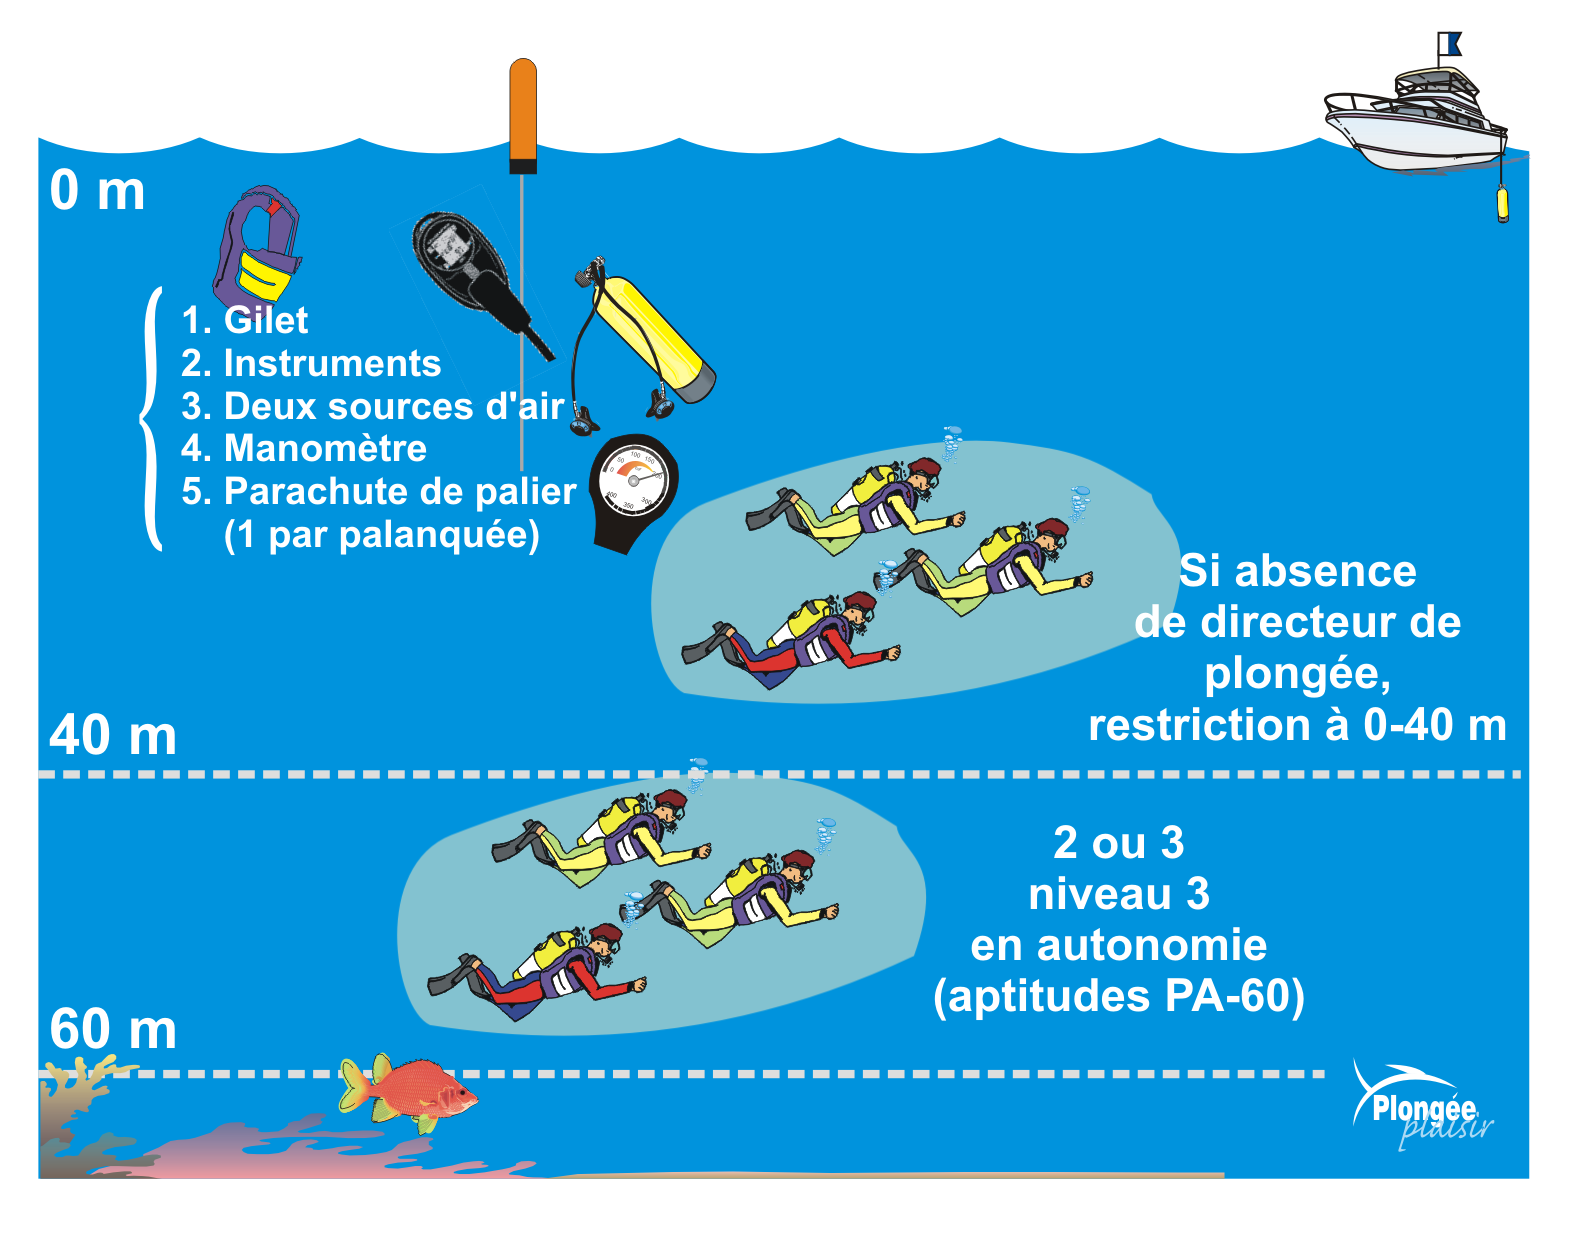
\includegraphics[height=0.9\textheight]{images/prerogative_n3}
\end{frame}

\begin{frame}{Les Prérogatives (Code du Sport)}
    \begin{block}{Le plongeur N3 FFESSM est :}
        \begin{itemize}
            \item \textbf{PA60} : Plongeur Autonome à 60m (si un DP est présent).
            \item \textbf{PA40} : Plongeur Autonome à 40m (en l'absence de DP).
            \item Équivalence CMAS 3*.
        \end{itemize}
    \end{block}

    \begin{alertblock}{Attention}
        \begin{itemize}
            \item Aucune équivalence directe avec PADI/SSI.
            \item Le RIFAP est un pré-requis obligatoire.
        \end{itemize}
    \end{alertblock}
\end{frame}

\begin{frame}{Matériel et Documents}
    \textbf{Matériel obligatoire (idem N2 + autonomie) :}
    \begin{itemize}
        \item Gilet.
        \item Instruments de décompression (ordinateur ou profondimètre + tables MN90).
        \item 2 sources d'air.
        \item Manomètre.
        \item Parachute de palier (1 par palanquée).
    \end{itemize}

    \vspace{0.5cm}
    \textbf{Documents nécessaires :}
    \begin{itemize}
        \item \textbf{Licence} : Assurance RC, valide du 01/09 au 31/12 (année suivante).
        \item \textbf{CACI} (Certificat Médical d'absence de contre-indication) : Moins d'un an dans les clubs associatifs.
        \item \textbf{Carnet de plongée} : Justifie l'expérience auprès des centres.
    \end{itemize}
\end{frame}

\begin{frame}{Responsabilité}
    \begin{block}{Responsabilité du Plongeur Autonome N3}
        En l'absence de DP, le plongeur N3 est responsable de :
        \begin{itemize}
            \item La planification de la plongée (site, profondeur, durée, DTR).
            \item La sécurité de la palanquée (matériel, procédures, secours).
            \item Le respect de la réglementation (prérogatives, matériel).
        \end{itemize}
    \end{block}

    \begin{alertblock}{Attention}
        Une mauvaise gestion peut engager votre responsabilité civile et \textbf{pénale} en cas d'accident.
    \end{alertblock}
\end{frame}

\begin{frame}{Responsabilités et Assurances}
    \centering
    
    \begin{tikzpicture}[
        scale=0.85, transform shape,
        % Styles globaux (Notez l'absence de lignes vides ici)
        base/.style={align=center, font=\small},
        % Style "Cause" (Haut)
        box_cause/.style={base, fill=FillCause, text=PrimaryColor, text width=3cm, minimum height=1.2cm, inner sep=5pt},
        % Style "Concept" (Milieu)
        box_concept/.style={base, fill=FillConcept, text=white, text width=3.2cm, minimum height=1.2cm, font=\bfseries\small},
        % Style "Description" (Bas)
        text_desc/.style={base, text=PrimaryColor, text width=3.5cm, node distance=1.5cm},
        % Style des flèches
        arrow/.style={->, >={Latex[length=3mm]}, thick, PrimaryColor},
        % Espacement global
        node distance=0.8cm and 0.3cm
    ]

    % --- COLONNE 1 (GAUCHE) ---
    \node[box_cause] (top1) {Infraction\\à la loi};
    \node[box_concept, below=of top1] (mid1) {Responsabilité\\pénale};
    \node[text_desc, below=of mid1] (bot1) {Pas d'assurance\\mais un contrat RC\\peut prévoir une\\protection juridique};

    % --- COLONNE 2 (CENTRE) ---
    \node[box_cause, right=of top1] (top2) {Préjudice causé\\à un tiers};
    \node[box_concept, below=of top2] (mid2) {Responsabilité\\civile};
    \node[text_desc, below=of mid2] (bot2) {Assurance en RC\\(dommages et\\intérêts)\\\textcolor{AlertColor}{\textbf{Obligatoire}}};

    % --- COLONNE 3 (DROITE) ---
    \node[box_cause, right=of top2, text width=3.5cm] (top3) {Dommages\\\textbf{corporels} sans\\tiers responsable};
    
    % Note : le "-|" permet d'aligner verticalement sous mid2 mais horizontalement avec top3
    \node[text_desc, below=of mid2 -| top3] (bot3) {Assurance individuelle\\Assistance, rapatriement\\[1em]\textcolor{AlertColor}{Facultatif en loisir}};

    % --- FLÈCHES ---
    \draw[arrow] (top1) -- (mid1);
    \draw[arrow] (mid1) -- (bot1);
    \draw[arrow] (top2) -- (mid2);
    \draw[arrow] (mid2) -- (bot2);
    \draw[arrow] (top3) -- (bot3);

    % --- ARRIÈRE-PLAN ---
    \begin{scope}[on background layer]
        \node[fit=(top1)(bot3)(top3), fill=CanvasBg, draw=PrimaryColor!50, inner sep=15pt, rounded corners=0pt] {};
    \end{scope}

    \end{tikzpicture}
\end{frame}

% ==============================================================================
% SECTION 2: CALCULS D'AUTONOMIE
% ==============================================================================
\section{Calculs d'Autonomie}

\begin{frame}{Introduction}
    La planification de la plongée nécessite des calculs d'autonomie précis 
    pour garantir la sécurité de la palanquée, surtout en absence de Directeur de Plongée (DP).
    \begin{block}{Objectifs}
        \begin{itemize}
            \item Comprendre la relation entre pression, volume et consommation d'air.
            \item Savoir calculer l'autonomie en fonction de la profondeur et de la consommation.
            \item Appliquer la règle des tiers pour une gestion sécurisée du gaz.
        \end{itemize}
    \end{block}
\end{frame}

% --- D. LES BOUTEILLES/ÉPROUVETTES (Volumes) ---
% Macro pour dessiner une bouteille
% #1: x, #2: y, #3: Hauteur remplissage (0 à 1), #4: Label Volume, #5: Label Math
\newcommand{\drawbottle}[5]{
    % #1: x, #2: y
    % #3: Volume d'AIR (1.0 = plein, 0.5 = moitié, 0.25 = quart)
    % #4: Texte Volume, #5: Texte Math
    
    \begin{scope}[shift={(#1,#2)}]
        % --- 1. LE REMPLISSAGE (L'EAU D'ABORD) ---
        % On remplit TOUT le volume possible en EAU (Cyan)
        % Le goulot (en bas) + le corps (en haut)
        % Comme ça, le bas ne sera jamais blanc.
        
        % Le Goulot (Trapèze du bas)
        \fill[cyan!40] (-0.1, -1) -- (0.1, -1) -- (0.3, -0.8) -- (-0.3, -0.8) -- cycle;
        
        % Le Corps principal (Rectangle) - On le remplit totalement d'eau par défaut
        \fill[cyan!40] (-0.3, -0.8) rectangle (0.3, 1);

        % --- 2. L'AIR (LE BLANC PAR DESSUS) ---
        % On calcule la hauteur d'AIR.
        % Hauteur totale du corps = 1.8 (de -0.8 à 1.0)
        % Hauteur Air = 1.8 * #3
        % Le rectangle d'air part du HAUT (1.0) et descend.
        \fill[white] (-0.28, 0.98) rectangle (0.28, {1.0 - (1.8 * #3)});

        % --- 3. LE CONTOUR (NOIR) ---
        % On redessine les traits noirs par dessus les couleurs
        \draw[thick, black] (-0.3, 1) -- (-0.3, -0.8) -- (-0.1, -1) -- (0.1, -1) -- (0.3, -0.8) -- (0.3, 1) -- cycle;
        % Petite courbe pour fermer le haut joliment (optionnel)
        %\draw[thick, black] (-0.3, 1) arc(180:0:0.3cm and 0.05cm); 

        % --- 4. TEXTES ---
        % Texte volume à droite
        \node[right, text=blue!80!black, font=\bfseries\small] at (0.4, 0) {#4};
        
        % Texte Math (= 12) loin à droite
        \node[right, text=black, font=\bfseries\large] at (4.5, 0) {= 12};
    \end{scope}
}

\begin{frame}{Rappels Physiques}
    \begin{columns}
        \begin{column}{0.6\textwidth}
            \centering
            \begin{tikzpicture}[
                scale=0.65, transform shape, % Ajuste la taille pour que ça rentre
                font=\sffamily\bfseries,
                % Définition des couleurs spécifiques à l'image
                colEau/.style={fill=cyan!30},
                colTerre/.style={fill=brown!60!black},
                colTexteRouge/.style={text=red, fill=white, inner sep=2pt, font=\bfseries},
                colBoite/.style={fill=white, text=blue!80!black, draw=blue!80!black, thin, inner sep=3pt},
                arrowStyle/.style={->, >=Latex, red, line width=4pt}
            ]

            % --- A. DÉCORS (Fond) ---
            % 1. L'EAU : On la fait commencer à x=0 pour qu'elle passe SOUS la falaise.
            % Plus de trou possible !
            \fill[cyan!20] (0, 0.5) rectangle (14, -7.5);
            
            % Surface de l'eau (Vagues)
            \draw[cyan!50, decorate, decoration={snake, amplitude=1.5pt, segment length=5pt}] (0, 0.5) -- (14, 0.5);

            % La Falaise (à gauche)
            \fill[brown!70!black] (-0.5,1) -- (2,1) -- (2.2, -0.5) -- (1.8, -2) -- (2, -4) -- (1.5, -7.5) -- (-0.5, -7.5) -- cycle;
            \node[text=blue!80!black, anchor=south west] at (-0.5, 0.5) {Surface};

            % --- B. LA FLÈCHE DE PRESSION (Axe central) ---
            % On trace une grande flèche rouge vers le bas
            \draw[arrowStyle] (4, 0.5) -- (4, -7);
            \node[text=red, align=center, font=\bfseries\small] at (4, 1) {P. Absolue\\1 bar};

            % --- C. LES ÉTAGES (Profondeur & Pression) ---
            
            % Niveau 10m
            \node[colBoite] at (1, -2) {10m};
            \node[colTexteRouge] at (4, -2) {2 bars};

            % Niveau 20m
            \node[colBoite] at (1, -4.5) {20m};
            \node[colTexteRouge] at (4, -4.5) {3 bars};

            % Niveau 30m
            \node[colBoite] at (1, -7) {30m};
            \node[colTexteRouge] at (4, -7) {4 bars};

            % Dessin des 4 bouteilles
            % Surface (0m) : 1 bar -> Vol 12 (100%)
            \drawbottle{7}{1}{1}{12 litres}{}
            
            % 10m : 2 bars -> Vol 6 (50%)
            \drawbottle{7}{-1.5}{0.5}{6 litres}{}
            
            % 20m : 3 bars -> Vol 4 (33%)
            \drawbottle{7}{-4}{0.33}{4 litres}{}
            
            % 30m : 4 bars -> Vol 3 (25%)
            \drawbottle{7}{-6.5}{0.25}{3 litres}{}

            \end{tikzpicture}
        \end{column}

        \begin{column}{0.35\textwidth}
            \begin{block}{Loi de Mariotte}
                Les volumes gazeux sont inversement proportionnels à la pression.
                $$ P \times V = \text{Constante} $$
                $$ P_1 \times V_1 = P_2 \times V_2 $$
            \end{block}
        \end{column}
    \end{columns}
\end{frame}

\begin{frame}{La Physique en application à l'autonomie}
    \begin{block}{Rappel}
        L'air délivré par le détendeur est ramené à la pression ambiante (ou absolue) 
        pour pouvoir être respiré sous l'eau.  
    \end{block}
    \begin{exampleblock}{Exemple de consommation (20L/min surface)}
        \begin{itemize}
            \item Surface (1 bar) : 20 L/min
            \item 10m (2 bars) : $20 \times 2 = 40$ L/min
            \item 20m (3 bars) : $20 \times 3 = 60$ L/min
        \end{itemize}
    \end{exampleblock}
    \begin{alertblock}{Attention}
        La consommation d'air augmente avec la profondeur. 
        Il est donc crucial de planifier ses plongées en tenant compte de l'autonomie.
    \end{alertblock}
\end{frame}

% --- FRAME 1 : EXERCICE (À afficher avant pour les élèves) ---
\begin{frame}{Exercice : Calcul d'Autonomie}
    \textbf{Données :}
    \begin{itemize}
        \item Plongeur avec un Bloc de \textbf{15 Litres} gonflé à \textbf{200 bars}.
        \item Consommation en surface estimée à \textbf{20 L/min}.
        \item On néglige la réserve pour cet exercice (Volume dispo $\approx$ \textbf{?} L).
    \end{itemize}
    
    \vspace{0.5cm}
    
    \textbf{À vous de jouer : complétez le tableau suivant.}
    
    \begin{table}[]
        \centering
        \renewcommand{\arraystretch}{1.5} % Agrandit les cases pour la lisibilité
        \begin{tabular}{cccc}
        \toprule
        \textbf{Prof.} & \textbf{Pression (Pabs)} & \textbf{Conso à Prof.} & \textbf{Autonomie} \\
        \midrule
        0 m    & 1 bar       & 20 L/min         & \textbf{?} \\ 
        \hline
        20 m   & \textbf{?}  & \textbf{?}       & \textbf{?} \\ 
        \hline
        40 m   & \textbf{?}  & \textbf{?}       & \textbf{?} \\ 
        \bottomrule
        \end{tabular}
    \end{table}
\end{frame}

% --- FRAME 2 : SOLUTION (Votre frame originale améliorée) ---
\begin{frame}{Solution : Calcul d'Autonomie}
    \begin{columns}
        \begin{column}{0.4\textwidth}
            $$ \text{Autonomie} = \frac{\text{Air disponible}}{\text{Consommation à prof.}} $$
        \end{column}
        \begin{column}{0.6\textwidth}
            \begin{exampleblock}{Rappel Données}
                Bloc 15L à 200b ($\approx$ 3000L). Conso surface : 20 L/min.
            \end{exampleblock}
        \end{column}
    \end{columns}

    \begin{table}[]
        \centering
        \renewcommand{\arraystretch}{1.3}
        \begin{tabular}{cccc}
        \toprule
        Prof. & Pression & Conso ($P \times 20$) & Autonomie \\
        \midrule
        0m    & 1b       & 20 L/min     & $3000 / 20 = \mathbf{150 \text{ min}}$ \\
        20m   & 3b       & 60 L/min     & $3000 / 60 = \mathbf{50 \text{ min}}$ \\
        40m   & 5b       & 100 L/min    & $3000 / 100 = \mathbf{30 \text{ min}}$ \\
        \bottomrule
        \end{tabular}
    \end{table}
    
    \begin{alertblock}{Constat}
        L'autonomie est divisée par 3 entre la surface et 20m !
        Plus on va profond, plus l'air se consomme vite.
    \end{alertblock}
\end{frame}

\begin{frame}{Astuce Pratique : La consommation au Palier (3m)}
    Comment estimer simplement sa consommation en bars pendant le palier ?
    
    \begin{block}{L'Astuce "Facile" (Règle du pouce)}
        Pour simplifier les calculs mentaux sous l'eau, retenez :
        \centering\Large\textbf{\textcolor{ffessmred}{2 bars par minute}}
    \end{block}

    \textbf{La Logique (Approximative) :}
    \begin{itemize}
        \item Consommation moyenne surface $\approx$ 20 L/min.
        \item À 3m (1,3 bar) $\rightarrow$ $20 \times 1,3 = 26$ L/min.
        \item \textbf{Bloc 15L} : $26 \div 15 \approx \mathbf{1,7}$ bar/min $\rightarrow$ Arrondi à \textbf{2 bars}.
        \item \textbf{Bloc 12L} : $26 \div 12 \approx \mathbf{2,1}$ bars/min $\rightarrow$ Arrondi à \textbf{2 bars}.
    \end{itemize}

    \begin{exampleblock}{Exemple concret}
        Pour un palier de \textbf{3 minutes} :
        $ 3 \text{ min} \times 2 \text{ bars/min} = \mathbf{6 \text{ bars consommés}} $
    \end{exampleblock}
\end{frame}

\begin{frame}{Planification et Gestion de l'Air (1/2)}

    % 1. L'Objectif de sécurité
    \begin{alertblock}{Objectif Prioritaire}
        En autonomie, la planification est indispensable pour \textbf{éviter la panne d'air}.
    \end{alertblock}

    \vspace{0.4cm}

    % 2. Les paramètres du calcul
    \textbf{Les 3 paramètres à prendre en compte :}
    \begin{enumerate}
        \item \textbf{Le Profil de la plongée} : La profondeur influe directement sur la consommation.
        \item \textbf{Le Volume de la bouteille} : La quantité d'air disponible au départ.
        \item \textbf{La Consommation du plongeur} : Un paramètre personnel et variable.
    \end{enumerate}

    \vspace{0.3cm}
\end{frame}

\begin{frame}{Planification et Gestion de l'Air (2/2)}
    % 3. La variabilité de la consommation (Note importante)
    \begin{block}{Attention à la consommation variable}
        Ce paramètre est difficile à évaluer car il évolue au cours de la plongée selon :
        \begin{itemize}
            \item \textbf{Le Froid}
            \item \textbf{Les Efforts} (courant, palmage, stabilisation)
            \item Le Stress
        \end{itemize}
    \end{block}

\end{frame}

\begin{frame}{Planification : La Règle des Tiers}
    Pour gérer sa sécurité et celle de la palanquée, on utilise souvent la règle des tiers pour gérer le gaz.

    \begin{columns}
        \column{0.5\textwidth}
        \begin{itemize}
            \item \textbf{1/3} : Pour l'aller / le fond.
            \item \textbf{1/3} : Pour le retour / la DTR.
            \item \textbf{1/3} : Sécurité (imprévus, assistance).
        \end{itemize}
       
        \column{0.5\textwidth}
        \begin{block}{Exemple (15L à 200b)}
            \begin{itemize}
                \item Air total : 3000 Litres.
                \item Air utilisable fond : 1000 Litres.
                \item À 40m (Conso 75L/min) :
                $$ 1000 / 75 \approx 13 \text{ min} $$
            \end{itemize}
        \end{block}
    \end{columns}

    \begin{alertblock}{Info Consommation}
        Si on n'a jamais mesuré sa consommation personnelle, on prend comme référence \textbf{15 L/min} (en surface).
    \end{alertblock}
\end{frame}

% ==============================================================================
% SECTION 3: BAROTRAUMATISMES
% ==============================================================================
\section{Les Barotraumatismes}

\begin{frame}{Définition et Généralités}
    \begin{block}{Rappels}
        En plongée, les volumes de gaz sont inversement proportionnels à la pression qu'ils subissent.
    \end{block}

    \vspace{0.3cm}

    \textbf{Définition :} Résultat du non-équilibre entre un volume gazeux du corps et la pression ambiante.
    
    \begin{itemize}
        \item \textbf{Facteur favorisant :} Variation RAPIDE de pression.
        \item \textbf{Zone à risque :} Proche de la surface (variations de volume importantes).
    \end{itemize}
    
    \textit{Le N3 doit savoir prévenir et gérer l'accident en l'absence de DP.}

    \vspace{0.4cm}
    
    \begin{block}{Résumé}
        Ils se caractérisent par leur effet immédiat et un facteur favorisant commun : une variation \textbf{rapide} de pression.
    \end{block}
\end{frame}

\begin{frame}{Attentes pédagogiques N3 — Barotraumatismes}
    Le plongeur Niveau 3 doit connaître les différents accidents barotraumatiques.\\
    Pour chacun d'eux, il doit :
    \begin{itemize}
        \item connaître la cause
        \item connaître les symptômes permettant de les détecter
        \item savoir les prévenir
        \item connaître l'ensemble de la conduite à tenir (CAT)
        \item être capable de répondre à des questions écrites ou orales en vue de l'examen
    \end{itemize}
\end{frame}

\begin{frame}{Surpression Pulmonaire — Schéma}
    \begin{columns}
        \column{0.7\textwidth}
        \centering
        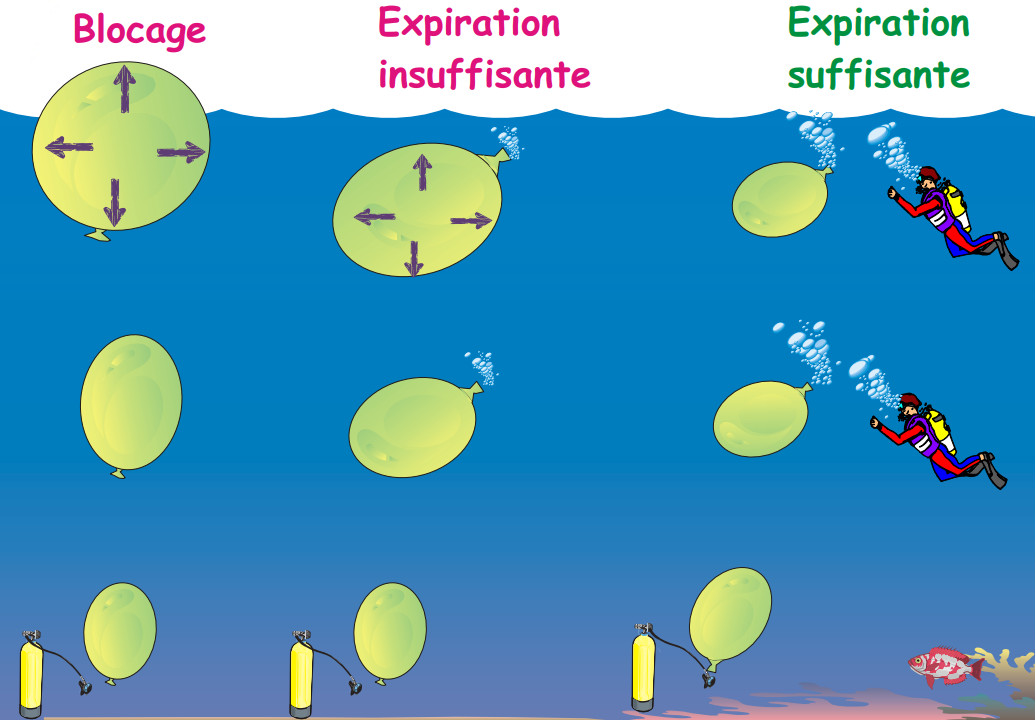
\includegraphics[height=0.85\textheight]{images/surpression_pulmonaire.png}

        \column{0.3\textwidth}
        \centering
        \small Schéma illustrant la surpression pulmonaire et l'expansion des gaz à la remontée.
    \end{columns}
\end{frame}

\begin{frame}{Surpression Pulmonaire — Conséquences}
    \begin{columns}
        \column{0.6\textwidth}
        \centering
        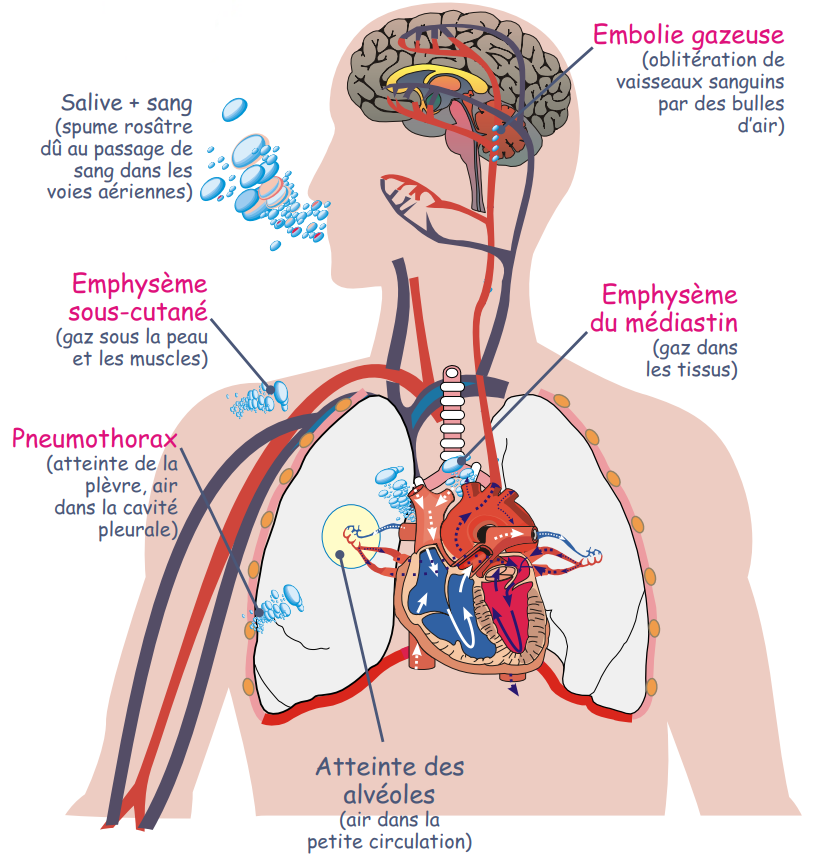
\includegraphics[height=0.85\textheight]{images/surpression_pulmonaire_consequences.png}

        \column{0.4\textwidth}
        \centering
        \small Principales conséquences de la surpression pulmonaire (embolie, emphysème, etc.).
    \end{columns}
\end{frame}

\begin{frame}{Surpression Pulmonaire - Résumé}
    \textbf{Cause :} Augmentation du volume pulmonaire au-delà de la tolérance (blocage respiration).
    
    \textbf{Symptômes :}
    \begin{itemize}
        \item Douleurs thoraciques.
        \item Difficultés respiratoires, crachats sanglants.
        \item Peut être fatal rapidement.
    \end{itemize}
    
    \textbf{Prévention N3 :}
    \begin{itemize}
        \item Gérer sa vitesse de remontée (ordinateur, bulles).
        \item Expiration continue à la remontée.
    \end{itemize}
\end{frame}

\begin{frame}{Surpression Pulmonaire — Conduite à Tenir (CAT)}
    \begin{columns}[T,totalwidth=\textwidth]
        \column{0.55\textwidth}
        \begin{itemize}
            \item \textbf{\textcolor{ffessmred}{Position}} confortable: \textbf{\textcolor{ffessmred}{demi-assise}} ou \textbf{\textcolor{ffessmred}{allongée}}.
            \item \textbf{\textcolor{ffessmred}{Déséquiper}} (bloc, stab, combi).
            \item \textbf{\textcolor{ffessmred}{Oxygène}}: \textbf{\textcolor{ffessmred}{15 L/min}} (masque haute concentration).
        \end{itemize}

        \column{0.45\textwidth}
        \begin{itemize}
            \item Si \textbf{\textcolor{ffessmred}{consciente}}: petites gorgées \textbf{\textcolor{ffessmred}{d'eau}}.
            \item \textbf{\textcolor{ffessmred}{Alerter}} les secours.
            \item \textbf{\textcolor{ffessmred}{Évacuation rapide}} (prise en charge type \textbf{\textcolor{ffessmred}{ADD}}).
        \end{itemize}
    \end{columns}
\end{frame}

\begin{frame}{Barotraumatisme de l'Oreille — Descente}
    \begin{columns}[T,totalwidth=\textwidth]
        \column{0.55\textwidth}
        \centering
        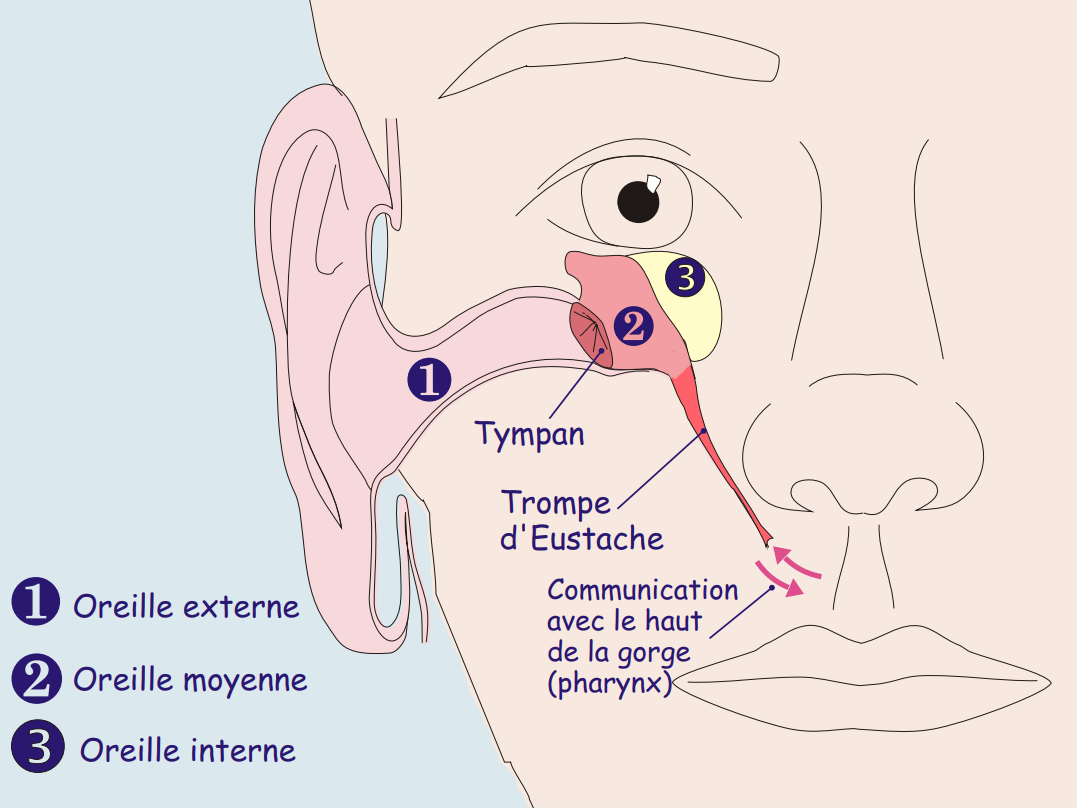
\includegraphics[height=0.8\textheight]{images/baro_oreille.png}

        \column{0.4\textwidth}
        \small
        \textbf{\textcolor{ffessmred}{Équilibrage}} régulier à la descente (Valsalva, déglutition).\\[0.5em]
        \textbf{Descente (Oreille moyenne)}
        \begin{itemize}
            \item \textit{Cause} : Non-équilibrage ou Valsalva tardif.
            \item \textit{Symptôme} : \textbf{\textcolor{ffessmred}{douleur aiguë}}.
            \item \textit{Prévention} : manœuvres \textbf{\textcolor{ffessmred}{douces et précoces}}, ne pas forcer.
            \item \textbf{\textcolor{ffessmred}{CAT}} : stopper la descente, corriger l'équilibrage.
        \end{itemize}

        \begin{alertblock}{Attention — \textbf{Coup de piston}}
            Forcer la \textbf{\textcolor{ffessmred}{Valsalva}} = surpression brutale
        \end{alertblock}
    \end{columns}
\end{frame}

\begin{frame}{Barotraumatisme de l'Oreille — Remontée}
    \begin{columns}[T,totalwidth=\textwidth]
        \column{0.55\textwidth}
        \centering
        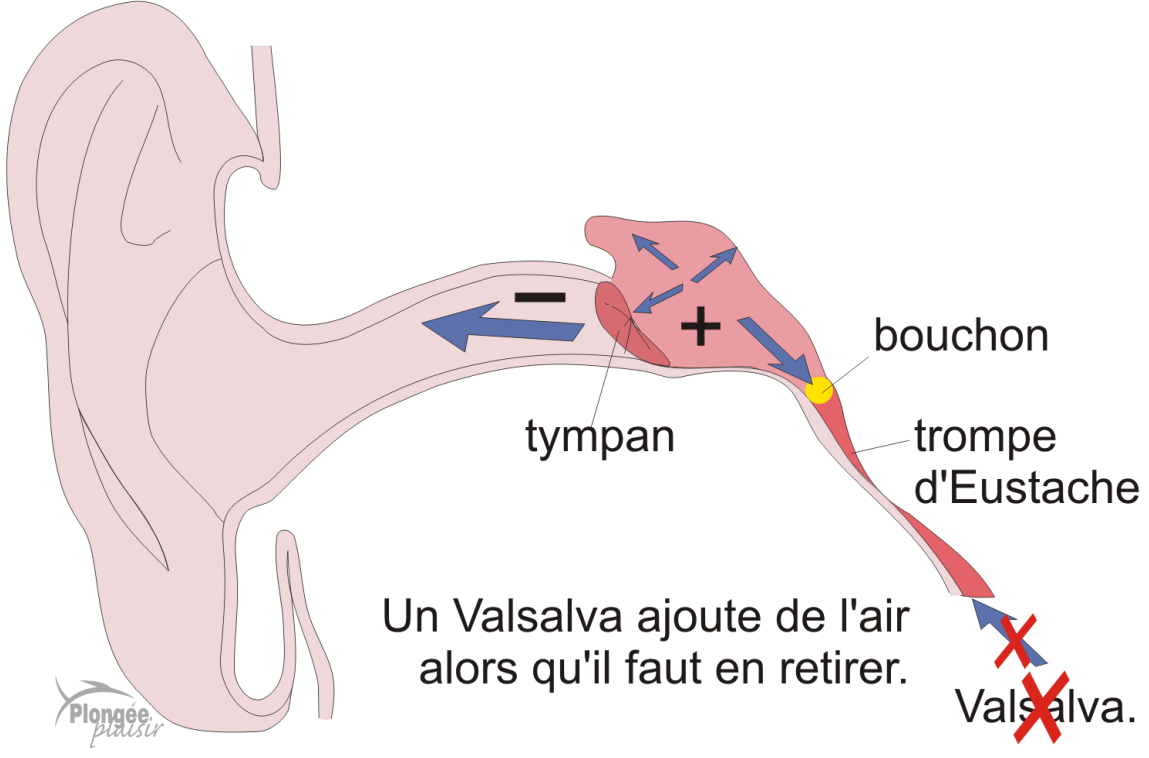
\includegraphics[height=0.7\textheight]{images/baro_oreille_vertige_alterno_barique.png}

        \column{0.4\textwidth}
        \small
        \textbf{Remontée (Vertige alterno-barique)}
        \begin{itemize}
            \item \textit{Cause} : Une oreille s'équilibre mal (bouchon, mucosité).
            \item \textit{Symptôme} : \textbf{\textcolor{ffessmred}{vertiges intenses}} à la remontée.
            \item \textit{Action} : \textbf{\textcolor{ffessmred}{redescendre un peu}}, déglutir, \textbf{\textcolor{ffessmred}{remonter lentement}}.
            \item \textbf{\textcolor{ffessmred}{Prévention}} : hygiène ORL, éviter de plonger enrhumé.
        \end{itemize}
        \begin{alertblock}{Attention — \textbf{Pas de Valsalva}}
            \textbf{\textcolor{ffessmred}{Valsalva}} = Surpression pulmonaire
        \end{alertblock}
    \end{columns}
\end{frame}

\begin{frame}{Vertige alterno-barique — \textbf{Symptômes} et \textbf{CAT}}
    \textbf{Symptômes} :
    \begin{itemize}
        \item Apparaissent \textbf{\textcolor{ffessmred}{sous l'eau}} pendant la \textbf{\textcolor{ffessmred}{remontée}} (différencier d'un \textbf{ADD} souvent \textbf{\textcolor{ffessmred}{à la sortie}}).
        \item \textbf{\textcolor{ffessmred}{Vertiges}} fugaces ou durables, parfois \textbf{\textcolor{ffessmred}{nausées}}.
        \item S'atténuent et \textbf{\textcolor{ffessmred}{disparaissent}} en quelques minutes après le retour à la surface.
    \end{itemize}

    \vspace{0.5em}
    \textbf{Conduite à Tenir (CAT)} :
    \begin{itemize}
        \item Maintenir une \textbf{\textcolor{ffessmred}{vigilance}} auprès du \textbf{\textcolor{ffessmred}{binôme}}.
        \item Conseiller une \textbf{\textcolor{ffessmred}{consultation ORL}} si \textbf{\textcolor{ffessmred}{douleur persistante}} à la sortie de l'eau.
    \end{itemize}
\end{frame}

\begin{frame}{Barotraumatisme des Sinus — Causes \& Mécanismes}
    \begin{columns}[T,totalwidth=\textwidth]
        \column{0.55\textwidth}
        \centering
        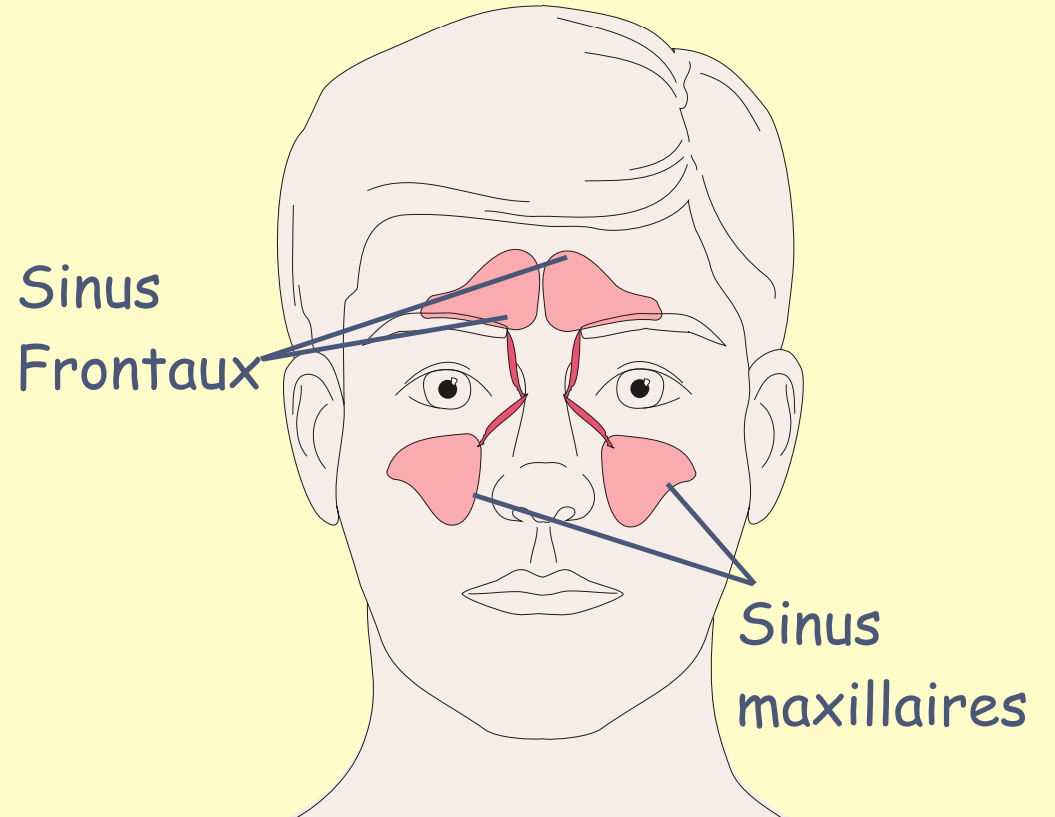
\includegraphics[height=0.75\textheight]{images/baro_sinus.png}

        \column{0.45\textwidth}
        \small
        Causes :
        \begin{itemize}
            \item Cavités de la face tapissées de \textbf{\textcolor{ffessmred}{muqueuse}}.
            \item \textbf{\textcolor{ffessmred}{Non-équilibre}} des sinus à la \textbf{descente} et à la \textbf{remontée}.
        \end{itemize}

        \vspace{0.4em}
        Mécanismes :
        \begin{itemize}
            \item \textbf{\textcolor{ffessmred}{Œdème / déformation}} de la muqueuse.
            \item \textbf{\textcolor{ffessmred}{Obstruction}} des ostia empêchant l'\textbf{\textcolor{ffessmred}{équilibrage}}.
        \end{itemize}
    \end{columns}
\end{frame}

\begin{frame}{Barotraumatisme des Sinus — Facteurs favorisants}
    \begin{block}{\textbf{Facteurs favorisants}}
        \begin{itemize}
            \item \textbf{\textcolor{ffessmred}{Vitesse}} de descente/remontée trop \textbf{\textcolor{ffessmred}{rapide}} si équilibrage difficile.
            \item En autonomie: adapter la \textbf{\textcolor{ffessmred}{vitesse}} pour tous; garder le \textbf{\textcolor{ffessmred}{dialogue}} binôme.
            \item \textbf{\textcolor{ffessmred}{Vasoconstricteurs}} déconseillés (effet court) → \textbf{\textcolor{ffessmred}{soucis d'équilibrage}} à la remontée.
        \end{itemize}
    \end{block}
\end{frame}

\begin{frame}{Barotraumatisme des Sinus — Symptômes \& CAT}
    Symptômes :
    \begin{itemize}
        \item Sinus \textbf{\textcolor{ffessmred}{encombrés}} (allergie, \textbf{\textcolor{ffessmred}{rhume}}) → air s'infiltre mal.
        \item \textbf{\textcolor{ffessmred}{Douleur faciale}} type « coup de poignard », parfois épistaxis (saignement de nez).
        \item Difficulté à s'\textbf{\textcolor{ffessmred}{équilibrer}} comme les fosses nasales.
    \end{itemize}

    \vspace{0.5em}
    Conduite à Tenir (CAT) :
    \begin{itemize}
        \item \textbf{\textcolor{ffessmred}{Ne pas faire}} d'équilibrage; \textbf{\textcolor{ffessmred}{stopper}} et \textbf{\textcolor{ffessmred}{ralentir}} la progression.
        \item \textbf{\textcolor{ffessmred}{Rincer}} les fosses nasales à l'eau de mer pour faciliter le passage de l'air.
        \item \textbf{\textcolor{ffessmred}{Ne pas plonger}} enrhumé; hygiène ORL.
        \item Consulter/demander un \textbf{\textcolor{ffessmred}{avis médical}} si gêne ou \textbf{\textcolor{ffessmred}{douleur persistante}} à la sortie de l'eau.
    \end{itemize}
\end{frame}

\begin{frame}{Placage de masque — Causes, Mécanismes}
    \begin{columns}[T,totalwidth=\textwidth]
        \column{0.55\textwidth}
        \centering
        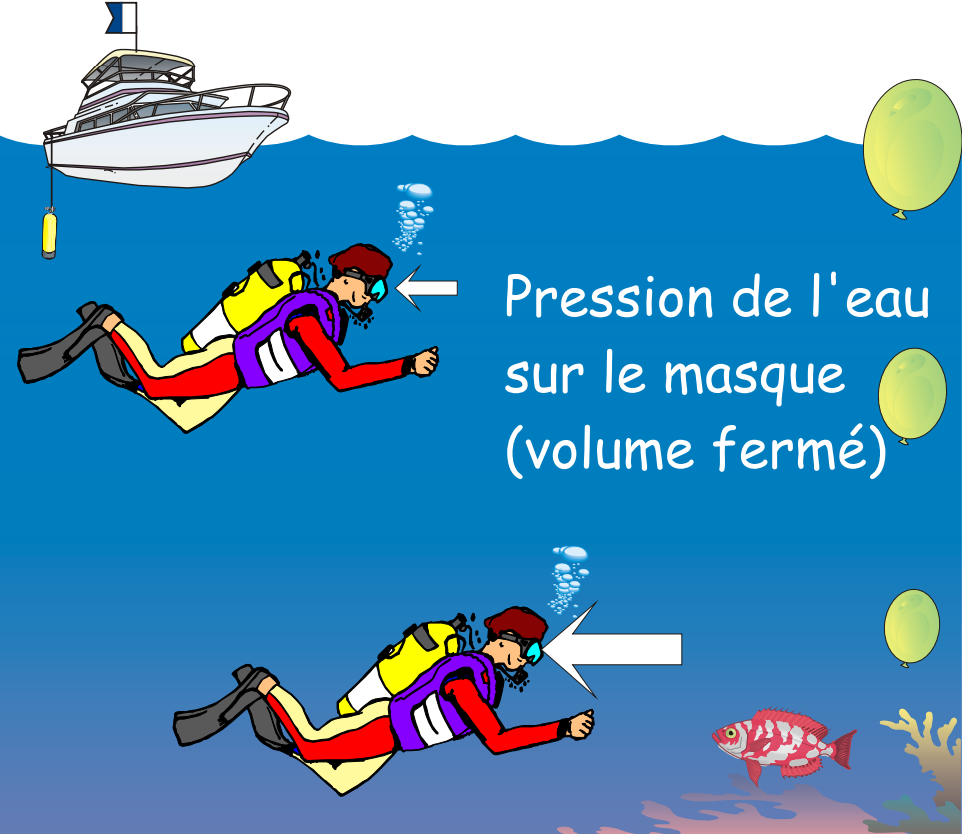
\includegraphics[height=0.75\textheight]{images/baro_masque.png}

        \column{0.45\textwidth}
        Cause :
        \begin{itemize}
            \item À la \textbf{descente}, \textbf{\textcolor{ffessmred}{non-équilibre}} du volume d'air du masque avec le milieu ambiant.
        \end{itemize}

        \vspace{0.3em}
        Mécanismes :
        \begin{itemize}
            \item \textbf{\textcolor{ffessmred}{Effet ventouse}} sur le visage.
            \item Le volume d'air entre la face et la vitre \textbf{varie} avec la \textbf{pression}.
            \item Avec l'\textbf{augmentation de pression}, le masque se \textbf{\textcolor{ffessmred}{plaque}} sur le visage.
        \end{itemize}
    \end{columns}
\end{frame}

\begin{frame}{Placage de masque — Symptômes, CAT}
    \vspace{0.3em}
    Facteurs favorisants :
    \begin{itemize}
        \item \textbf{\textcolor{ffessmred}{Sangle trop serrée}} (moins d'élasticité de la jupe).
        \item \textbf{\textcolor{ffessmred}{Vitesse}} de descente \textbf{rapide}.
    \end{itemize}

    \vspace{0.3em}
    Symptômes :
    \begin{itemize}
        \item Troubles de la \textbf{\textcolor{ffessmred}{vue}}, lésions légères \textbf{yeux/nez} (non graves, non irréversibles).
    \end{itemize}

    \vspace{0.3em}
    Conduite à Tenir (CAT) :
    \begin{itemize}
        \item \textbf{\textcolor{ffessmred}{Souffler par le nez}} à la descente pour \textbf{\textcolor{ffessmred}{équilibrer}} le masque.
        \item \textbf{\textcolor{ffessmred}{Adapter}} la vitesse et \textbf{\textcolor{ffessmred}{desserrer}} légèrement la sangle si besoin.
        \item \textbf{\textcolor{ffessmred}{Avis médical}} si gêne/douleur \textbf{\textcolor{ffessmred}{persistante}} à la sortie de l'eau.
    \end{itemize}
\end{frame}

\begin{frame}{Autres Barotraumatismes}
    \begin{itemize}
        \item \textbf{\textcolor{ffessmred}{Estomac/Intestin}} :
        \begin{itemize}
            \item Accident \textbf{rare} chez le plongeur actuel; concernait surtout les \textbf{scaphandriers « pieds lourds »} (alimentation abondante).
            \item Gaz digestifs qui se \textbf{dilatent} à la remontée → gêne/douleur.
            \item \textbf{Prévention/CAT} : éviter repas lourds avant plongée, \textbf{ralentir} si gêne, \textbf{évacuer l'air} si possible.
        \end{itemize}

        \vspace{0.4em}
        \item \textbf{\textcolor{ffessmred}{Dents}} :
        \begin{itemize}
            \item \textbf{Descente} : gencives \textbf{fragiles} plus sensibles (pression, froid de l'air détendu) → \textbf{remonter} et \textbf{stopper}.
            \item \textbf{Remontée} : poche d'air sous \textbf{dent cariée/mal soignée} → \textbf{douleur croissante}.
            \item \textbf{Prévention} : \textbf{bonne hygiène dentaire}.
            \item \textbf{CAT} : \textbf{stopper} la progression; si douleur, \textbf{redescendre 1–2 m} puis \textbf{remonter lentement}; \textbf{consulter} si douleur persistante.
        \end{itemize}
    \end{itemize}
\end{frame}

\begin{frame}{Synthèse des Barotraumatismes}
    \centering
    \renewcommand{\arraystretch}{1.4} % Aère le tableau
    \footnotesize % Réduit légèrement la police pour que tout rentre
    
    \begin{table}[]
        \begin{tabular}{p{2cm} c p{3.5cm} p{3.5cm}}
        \toprule
        \textbf{Type} & \textbf{Qd?} & \textbf{Prévention Clé} & \textbf{Conduite à Tenir (CAT)} \\ 
        \midrule
        
        \textbf{Surpression Pulmonaire} & $\nearrow$ & 
        Expiration continue \newline Vitesse contrôlée & 
        \textbf{Urgence Vitale !} \newline O2 (15L/min) + Évacuation \\ 
        \hline
        
        \textbf{Oreilles \newline \& Sinus} & $\searrow$ \newline $\nearrow$ & 
        Manœuvres douces \newline Ne jamais forcer \newline Vitesse lente & 
        Stopper l'immersion \newline Consulter ORL si douleur persistante \\ 
        \hline
        
        \textbf{Dents} & $\searrow \nearrow$ & 
        Hygiène dentaire \newline Stop si douleur & 
        Consultation dentiste \\ 
        \hline
        
        \textbf{Masque} & $\searrow$ & 
        Souffler par le nez & 
        - \\ 
        \hline
        
        \textbf{Intestins} & $\nearrow$ & 
        Alimentation saine \newline Évacuer les gaz & 
        Consultation si douleur \\ 
        
        \bottomrule
        \end{tabular}
    \end{table}

    \vspace{0.2cm}
    \scriptsize{Légende : $\searrow$ Descente \quad $\nearrow$ Remontée}
\end{frame}

% ==============================================================================
% SECTION 4: ACCIDENT DE DESATURATION (ADD)
% ==============================================================================
\section{L'Accident de Désaturation (ADD)}

\begin{frame}{Attentes pédagogiques N3 — ADD}
    Dans le cadre de leurs nouvelles prérogatives, les plongeurs N3 évoluent jusqu'à \textbf{60 mètres}.\\
    Cette zone profonde accroît les risques ; les connaissances en prévention, organisation et secours doivent donc être approfondies.

    \vspace{1em}
    À propos de l'\textbf{accident de décompression}, le futur Niveau 3 doit :
    \begin{itemize}
        \item Connaître les \textbf{causes}.
        \item Identifier les \textbf{symptômes} pour le détecter en l'absence de Guide de Palanquée (GP).
        \item Savoir le \textbf{prévenir}.
        \item Maîtriser la \textbf{Conduite à Tenir (CAT)}.
        \item Être capable de répondre aux questions (écrites/orales) de l'examen.
    \end{itemize}
\end{frame}

\begin{frame}{Mécanisme de l'ADD — Principe}
    \begin{block}{Principe Physique : Loi de Henry}
        À température constante, la quantité de gaz dissous dans un liquide est proportionnelle à la pression au-dessus du liquide.
        \[ \text{Quantité de gaz} = \text{Coefficient} \times \text{Pression} \]
    \end{block}

    \vspace{1em}
    \textbf{Le problème en plongée :}
    \begin{itemize}
        \item À la descente, l'azote se dissout dans les tissus (\textbf{sous saturation}).
        \item À la remontée, la pression diminue, l'azote doit être évacué.
        \item Si la remontée est \textbf{trop rapide} ou l'élimination perturbée, des bulles se forment (effet bouteille de champagne) et bloquent la circulation.
    \end{itemize}
\end{frame}

\begin{frame}{Rappels de Physiologie — Échanges Gazeux}
    \begin{columns}[T,totalwidth=\textwidth]
        \column{0.5\textwidth}
        \centering
        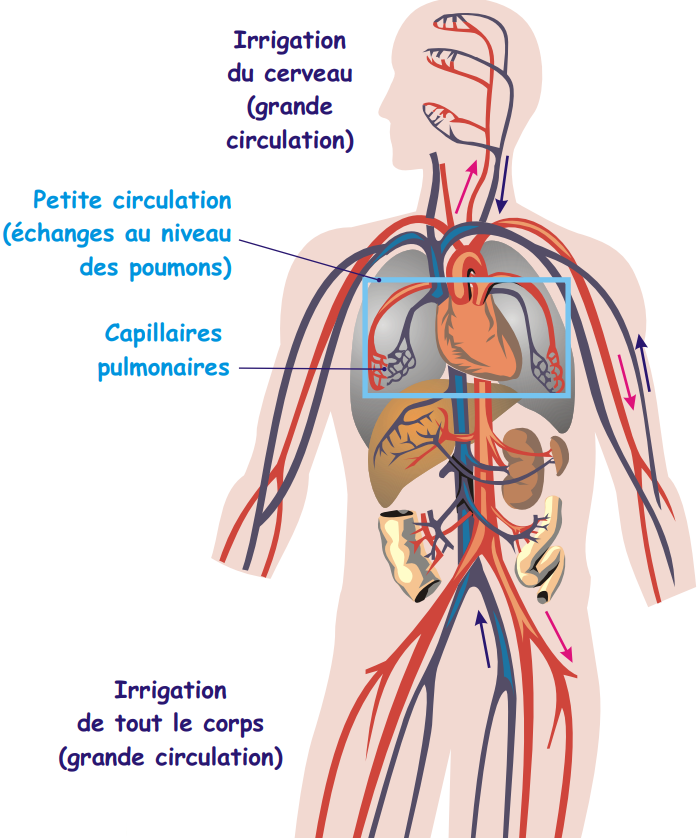
\includegraphics[height=0.85\textheight]{images/add_circulation.png}

        \column{0.5\textwidth}
        \small
        \textbf{\textcolor{ffessmred}{Oxygène ($O_2$)}} \\
        Carburant de l'organisme, inspiré via l'air.
        
        \vspace{0.8em}
        \textbf{\textcolor{ffessmred}{Dioxyde de Carbone ($CO_2$)}} \\
        Déchet du travail musculaire, éliminé à l'expiration.
        
        \vspace{0.8em}
        \textbf{Mécanisme}
        \begin{itemize}
            \item \textbf{Échanges} gazeux (O$_2$/CO$_2$/N$_2$) au niveau des \textbf{alvéoles pulmonaires}.
            \item \textbf{Transport} : Le sang véhicule les gaz entre les poumons et toutes les cellules via le \textbf{système circulatoire}.
        \end{itemize}
    \end{columns}
\end{frame}

% --- DÉFINITIONS GLOBALES ---
% (À laisser ici ou dans le préambule de main.tex)
\tikzset{
    box_double/.style={
        rectangle split,
        rectangle split parts=2,
        rectangle split part fill={yellow, white},
        draw=black, thick,
        align=center,
        minimum width=1.8cm,
        minimum height=1.6cm
    },
    star_alert/.style={
        star, star points=9, star point ratio=1.4,
        draw=red, fill=red, text=black,
        align=center, font=\bfseries\scriptsize,
        inner sep=2pt
    },
    arrow/.style={->, >=Latex, thin, black},
    bubble/.style={
        ellipse, draw=black, fill=white,
        align=center, font=\scriptsize, inner sep=2pt
    }
}

\newcommand{\drawstate}[5]{
    \node[box_double] (#1) at (#2, #3) {
        #4
        \nodepart{two}
        #5
    };
}

\begin{frame}{Le mécanisme de saturation}
    \centering
    
    \begin{tikzpicture}[
        scale=0.5, transform shape,
        font=\sffamily\bfseries
    ]

    % --- A. LE PROFIL ---
    \draw[line width=2pt] 
        (-2, 0) -- (-1, 0)       % DEPART : Une ligne horizontale en surface (de gauche à droite)
        -- (2, -6)              % DESCENTE : On descend jusqu'à Y=-6 (le fond)
        -- (9, -6)              % FOND : On reste à -6 jusqu'à X=8 (ligne plate)
        -- (11, -4)             % REMONTÉE : On remonte jusqu'à -4 (premier palier)
        -- (13, -4)             % PALIER 1 : On reste stable à -4 pendant 2 unités
        -- (14, -2)             % REMONTÉE : On remonte jusqu'à -2 (deuxième palier)
        -- (16, -2)             % PALIER 2 : On reste stable à -2
        -- (17, 0) -- (20, 0);  % SORTIE : On remonte en surface (0) et on nage un peu.
    \draw[line width=2pt, dashed] (11, -4) -- (12, 1);

    % --- B. LES ÉTATS ---
    \drawstate{s1}{2}{1}{++}{++}
    \node[left=0.2cm of s1, align=right] {Saturation};

    \drawstate{s2}{2}{-3}{++++}{++}
    \node[left=1cm of s2, align=right] {Sous\\Saturation};

    \drawstate{s3}{3.5}{-7.5}{++++++}{++++}
    \node[left=0.2cm of s3, align=right] {Sous\\Saturation};
    
    \drawstate{s4}{7.5}{-7.5}{++++++}{++++++}
    \node[below=0.2cm of s4] {Saturation};
    
    \drawstate{s5}{11}{-3}{++++}{+++++}

    \drawstate{s6}{15}{-1}{+++}{+++++}
    \node[right=0.5cm of s6] {Sur-Saturation};

    \drawstate{s7}{18}{1}{++}{++++}
    \node[right=0.2cm of s7] {Sur-Saturation};

    % --- 7. ACCIDENT ---
    % 1. On dessine D'ABORD la boîte s7 pour qu'elle existe
    \drawstate{s8}{12}{1}{++}{+++++}
    
    % 2. On dessine l'étoile DERRIÈRE (sur le calque 'background')
    % Cela nécessite \usetikzlibrary{backgrounds} dans main.tex
    \begin{scope}[on background layer]
        \node[star_alert, fit=(s8), scale=1] {}; 
    \end{scope}

    \node[right=0.1cm of s8, align=left, font=\bfseries\tiny] {Sur-Saturation\\Critique !!!};


    % --- C. FLÈCHES ---
    \draw[arrow] (s1.south) -- (s2.north);
    \draw[arrow] (s2.south) -- (s3.north);
    \draw[arrow] (s3.east) -- (s4.west);
    \draw[arrow] (s4.north) -- (s5.south);
    \draw[arrow] (s5.north) -- (s8.south);
    \draw[arrow] (s5.north) -- (s6.south);
    \draw[arrow] (s6.north) -- (s7.south);

    % --- D. LÉGENDE ---
    \node[bubble, fill=yellow, text width=2cm] (explYellow) at (13, -5.5) 
        {Pression\\partielle\\de N2\\dans l'air\\respiré};
    \node[bubble, text width=2.5cm] (explWhite) at (16, -7) 
        {N2 dissous\\dans le corps\\du plongeur};

    \draw[->, thin] (explYellow) -- (s4.one east);
    \draw[->, thin] (explWhite) -- (s4.two east);

    \end{tikzpicture}
\end{frame}

\begin{frame}{Cause et Mécanismes de l'ADD — Synthèse}
    \textbf{\textcolor{ffessmred}{Mécanismes}} :
    \begin{enumerate}
        \item \textbf{Reprise gazeuse} : À la remontée (baisse de pression), l'azote stocké repasse à l'état gazeux.
        \item \textbf{Évacuation} : Il quitte les tissus vers le sang, direction les poumons pour être expiré.
        \item \textbf{Blocage} : Si l'évacuation est perturbée (mauvais comportement, bulles trop volumineuses), l'azote s'accumule et \textbf{bloque la circulation}.
        \item \textbf{Conséquence} : Les tissus en aval ne sont plus oxygénés, occasionnant des \textbf{dommages} divers.
    \end{enumerate}

    \vspace{0.8em}

    \textbf{\textcolor{ffessmred}{Cause}} :
    \begin{itemize}
        \item \textbf{Blocage} de la circulation par des \textbf{\textcolor{ffessmred}{bulles d'azote}} dans le système sanguin lors de la désaturation.
    \end{itemize}
\end{frame}

\begin{frame}{Prévention de l'ADD — Principes Généraux}
    La prévention ne se limite pas au respect des tables.
    
    \begin{itemize}
        \item \textbf{Objectif} : Minimiser autant que possible les \textbf{\textcolor{ffessmred}{facteurs favorisants}}.
        \item \textbf{Responsabilité N3} : En autonomie, vous devez être particulièrement attentif pour \textbf{\textcolor{ffessmred}{modérer sa plongée}}.
        \item \textbf{Stratégie} : Limiter la \textbf{\textcolor{ffessmred}{charge en azote}} pour aller dans le sens de la sécurité.
    \end{itemize}

    \vspace{0.5em}
    \begin{block}{Règle d'or}
        Adopter un comportement adéquat \textbf{Avant}, \textbf{Pendant} et \textbf{Après} la plongée.
    \end{block}
\end{frame}

\begin{frame}{Prévention — Avant et Pendant}
    \textbf{Avant la plongée} :
    \begin{itemize}
        \item Ne pas plonger si \textbf{\textcolor{ffessmred}{fatigué}} ou sans envie.
        \item Vérifier la compatibilité des \textbf{\textcolor{ffessmred}{traitements médicaux}}.
    \end{itemize}

    \vspace{0.5em}
    \textbf{Pendant la plongée} :
    \begin{itemize}
        \item \textbf{\textcolor{ffessmred}{Effort}} et \textbf{\textcolor{ffessmred}{Froid}} : À limiter impérativement (augmentent la saturation).
        \item \textbf{\textcolor{ffessmred}{Profil}} : Éviter les profils \textbf{\textcolor{ffessmred}{Yoyo}} ou \textbf{\textcolor{ffessmred}{Inversés}}.
        \item \textbf{\textcolor{ffessmred}{Vitesse}} : Respect strict de la vitesse de remontée.
        \item \textbf{\textcolor{ffessmred}{Valsalva}} : Ne jamais faire de manœuvre force/prolongée à la remontée (gêne l'élimination pulmonaire).
    \end{itemize}
\end{frame}

\begin{frame}{Prévention — Après et Facteurs Individuels}
    \textbf{Après la plongée} (La désaturation continue en surface !) :
    \begin{itemize}
        \item Pas d'\textbf{\textcolor{ffessmred}{effort}} intense ("Sport" après plongée).
        \item Pas d'\textbf{\textcolor{ffessmred}{apnée}} (perturbe les échanges, attendre \textbf{au moins 6h}).
        \item Pas d'\textbf{\textcolor{ffessmred}{altitude}} (Montagne/Avion) : Planifier sa journée.
    \end{itemize}
    
    \vspace{0.5em}
    \textbf{Facteurs Physiologiques} (Facteurs de risque intrinsèques) :
    \begin{itemize}
        \item L'\textbf{\textcolor{ffessmred}{âge}}, la forme physique (surpoids).
        \item Le \textbf{\textcolor{ffessmred}{tabagisme}} (mauvaise vascularisation).
        \item L'\textbf{\textcolor{ffessmred}{alcool}}, la drogue, les médicaments.
    \end{itemize}
\end{frame}

\begin{frame}{Symptômes de l'ADD}
    Peuvent apparaître dès la sortie ou plusieurs heures après.
    
    \begin{alertblock}{Signes d'alerte}
        \begin{itemize}
            \item \textbf{Fatigue intense} (anormale).
            \item Troubles cutanés ("Puces", moutons).
            \item Troubles neurologiques : Fourmillements, paralysies, troubles sensitifs (vue, ouïe).
            \item Vertiges, nausées.
            \item Douleurs articulaires.
        \end{itemize}
        \textbf{\textcolor{ffessmred}{Règle d'or}} : Toute sensation anormale ou trouble (douleur dos, élocution, prostration...) 
        doit être \textbf{\textcolor{ffessmred}{considérée avec sérieux}} et traitée comme un ADD.
    \end{alertblock}
    \textit{Surveillance mutuelle impérative après la plongée !}
\end{frame}


\begin{frame}{Conduite à Tenir (CAT) - RIFAP}
    En l'absence de DP, le N3 prend en charge les secours :
    
    \begin{enumerate}
        \item \textbf{Sortir et Allonger} la victime (ne pas surélever les jambes).
        \item \textbf{Oxygène pur} : Inhalation à 15 L/min (le plus tôt possible).
        \item \textbf{Hydratation} : Faire boire de l'eau plate (si conscient) $\sim$ 1 Litre.
        \item \textbf{Alerte} : CROSS, Pompiers ou le SAMU.
        \item \textbf{Évacuation} : Organiser le transfert vers un caisson hyperbare.
        \item \textbf{Fiche d'évacuation} : Noter les paramètres de la plongée pour les médecins.
        \item \textbf{Surveillance} : Mettre à l'ombre, couvrir la victime et maintenir une surveillance.
    \end{enumerate}
\end{frame}

% ==============================================================================
% SECTION 5: CONCLUSION
% ==============================================================================
\section{Conclusion}
\begin{frame}{Synthèse de la 1ère Partie}
    \begin{block}{Ce qu'il faut retenir :}
        \begin{itemize}
            \item \textbf{Prérogatives :} PA60 (avec DP) et PA40 (sans DP). Vous devez connaître vos limites réglementaires.
            \item \textbf{Gestion d'air :} L'autonomie diminue drastiquement avec la profondeur. La \textbf{règle des tiers} est votre assurance vie.
            \item \textbf{Barotraumatismes :} La variation de pression est rapide près de la surface. Vigilance à la descente comme à la remontée.
            \item \textbf{ADD :} Le respect des procédures ne suffit pas toujours. Il faut combattre les facteurs favorisants (froid, effort, profil).
        \end{itemize}
    \end{block}

    \begin{center}
        \large \textbf{Le Niveau 3 est le niveau de l'autonomie complète.} \\
        \vspace{0.5em}
        \textit{Votre sécurité dépend de votre planification et de votre capacité à réagir.}
    \end{center}
\end{frame}

\begin{frame}{Vers la 2ème Partie...}
    Nous avons vu les risques et la théorie.
    
    Dans la seconde partie, nous aborderons la pratique de l'autonomie :
    \begin{itemize}
        \item Comment utiliser son ordinateur et gérer la décompression ?
        \item Comment s'organiser matériellement (bateau, sécu) ?
        \item Comment planifier concrètement la plongée ?
    \end{itemize}
\end{frame}

\begin{frame}
    \centering
    \Huge \textbf{Des questions ?}
\end{frame}

% ==========================================
% PARTIE 2
% ==========================================
\part{Théorie N3 - 2ème Partie\\Décompression, Intoxications, Froid, Organisation}

\section{Rappels Partie 1}

% --- FRAME 1 : RAPPELS RÉGLEMENTATION & PHYSIQUE ---
\begin{frame}{Rappels : Cadre et Principes}
    Avant d'aborder la suite, rappelons les fondamentaux du Niveau 3 :

    \begin{columns}
        \column{0.5\textwidth}
        \begin{block}{Prérogatives N3}
            \begin{itemize}
                \item \textbf{PA60} : Autonome jusqu'à 60m (avec DP).
                \item \textbf{PA40} : Autonome jusqu'à 40m (sans DP).
                \item \textbf{Responsable} de sa planification et de sa sécurité.
            \end{itemize}
        \end{block}

        \column{0.4\textwidth}
        \begin{block}{Physique (Loi de Mariotte)}
            $$ P \times V = \text{Constante} $$
            La pression augmente de \textbf{1 bar tous les 10m}.
            \begin{itemize}
                \item À 20m ($P_{abs}=3b$) : Consommation $\times 3$.
                \item Autonomie divisée par 3 !
            \end{itemize}
        \end{block}
    \end{columns}
    
    \vspace{0.5cm}
    \textbf{Règle d'or en autonomie :} On planifie \textbf{avant} de s'immerger (Air, Temps, Profondeur, Palanquée).
\end{frame}

% --- FRAME 2 : RAPPELS RISQUES ---
\begin{frame}{Rappels : Les Risques Majeurs}
    \begin{alertblock}{Barotraumatismes (Volumes gaz du corps)}
        \textbf{Cause :} Variation de pression (surtout 0-10m).
        \begin{itemize}
            \item \textbf{Surpression Pulmonaire ($\nearrow$)} : Expiration continue obligatoire.
            \item \textbf{Oreilles ($\searrow$)} : Manœuvres douces, ne jamais forcer.
        \end{itemize}
    \end{alertblock}

    \begin{block}{Accident de Désaturation (ADD - Loi de Henry)}
        \textbf{Cause :} Bulles d'azote bloquant la circulation.
        \begin{itemize}
            \item \textbf{Facteurs favorisants} : Profil, Froid, Effort, Age.
            \item \textbf{Prévention} : Respect vitesse remontée, hydratation, pas d'effort après.
            \item \textbf{CAT} : O2 (15L/min) + Évacuation + Eau.
        \end{itemize}
    \end{block}
\end{frame}

% --- FRAME 3 : EXERCICE AVANCÉ ---
\begin{frame}{Exercice de Planification (Niveau N3)}
    \textbf{Scénario :}
    Plongée sur une épave à \textbf{30 mètres}.
    \begin{itemize}
        \item Bloc de \textbf{15 Litres} gonflé à \textbf{210 bars}.
        \item Consommation surface (stress inclus) : \textbf{25 L/min}.
        \item Réserve de sécurité obligatoire : \textbf{50 bars}.
    \end{itemize}

    \vspace{0.3cm}
    \textbf{Calculez votre autonomie au fond selon 3 méthodes :}
    \begin{enumerate}
        \item \textbf{Méthode "Naïve"} : On consomme tout le gaz utilisable au fond (sans penser à la remontée).
        \item \textbf{Méthode "Réaliste"} : On déduit le gaz nécessaire à la remontée (DTR).
        \textit{\small(Pour l'exercice, on estime la consommation de la remontée à \textbf{400 Litres}).}
        \item \textbf{Méthode "Sécurisée"} : On applique la \textbf{Règle des Tiers}.
    \end{enumerate}
\end{frame}

% --- FRAME 4 : SOLUTION ---
% --- SOLUTION PARTIE 1 : SIMPLIFIÉE ---
\begin{frame}{Solution 1 : Méthode "Naïve"}
    \textit{"Je reste au fond tant que je n'ai pas atteint ma réserve."}
    
    \begin{enumerate}
        \item \textbf{Calcul de la Conso Fond ($C_{fond}$)} :
        $$ P_{abs} = 4 \text{ bars} \quad \Rightarrow \quad C_{fond} = 25 \times 4 = \mathbf{100 \text{ L/min}} $$
        
        \item \textbf{Gaz Utilisable :}
        $$ 210b - 50b (\text{Réserve}) = 160b $$
        $$ 160b \times 15L = \mathbf{2400 \text{ Litres}} $$
        
        \item \textbf{Autonomie :}
        $$ \text{Temps} = \frac{2400}{100} = \mathbf{24 \text{ minutes}} $$
    \end{enumerate}
    
    \begin{alertblock}{Danger}
        Si vous restez 24 min, vous entamez la remontée avec 50 bars.
        Vous arriverez en surface \textbf{dans la réserve} (car vous allez consommer en remontant). \textbf{C'est risqué.}
    \end{alertblock}
\end{frame}

% --- SOLUTION PARTIE 2 : AVEC DTR ---
\begin{frame}{Solution 2 : Intégration de la DTR}
    \textit{"Je garde du gaz pour remonter sereinement."}
    
    \begin{itemize}
        \item \textbf{Gaz Utilisable Total} : 2400 Litres (cf. calcul précédent).
        \item \textbf{Besoin Remontée (DTR)} : 400 Litres (Donnée exercice).
    \end{itemize}
    
    $$ \text{Gaz Dispo Fond} = 2400 - 400 = \mathbf{2000 \text{ Litres}} $$
    
    \textbf{Nouvelle Autonomie :}
    $$ \frac{2000}{100} = \mathbf{20 \text{ minutes}} $$
    
    \begin{block}{Constat}
        On perd 4 minutes de temps fond, mais on sort de l'eau avec la réserve intacte (50b). C'est la procédure standard minimale.
    \end{block}
\end{frame}

% --- SOLUTION PARTIE 3 : TIERS ---
\begin{frame}{Solution 3 : La Règle des Tiers}
    \textit{"Je consomme 1/3 à l'aller, 1/3 au retour, 1/3 sécurité."}
    \begin{columns}
        \column{0.4\textwidth}
        \begin{enumerate}
            \item \textbf{Calcul du Tiers (en pression) :}
            $$ \frac{210 \text{ bars}}{3} = \mathbf{70 \text{ bars}} $$
            
            \item \textbf{Volume disponible (1/3) :}
            $$ 70 \text{ bars} \times 15L = \mathbf{1050 \text{ Litres}} $$
            
            \item \textbf{Autonomie (Demi-tour) :}
            $$ \frac{1050}{100} \approx \mathbf{10 \text{ minutes}} $$
        \end{enumerate}

        \column{0.5\textwidth}
        \begin{exampleblock}{Comparaison Finale à 30m}
            \begin{itemize}
                \item Calcul simpliste : \textbf{24 min} (Dangereux)
                \item Calcul DTR : \textbf{20 min} (Standard)
                \item Règle des Tiers : \textbf{10 min} (Très sécurisé)
            \end{itemize}
        \end{exampleblock}
    \end{columns}
\end{frame}
\section{Les Intoxications Gazeuses}

\begin{frame}{La Narcose — Distinguer Effets et Crise}
    \textbf{Cause :} Augmentation de la $PpN_2$ (Loi de Dalton) perturbant le système nerveux.
    
    \textbf{Une distinction fondamentale pour le N3 :}
    \begin{itemize}
        \item \textbf{\textcolor{ffessmred}{Les Effets :}} Ressentis dès 30m. Modification physiologique sans danger immédiat si gérée.
        \item \textbf{\textcolor{ffessmred}{La Crise :}} Généralement au-delà de 40m. Modifications notables du comportement menaçant la sécurité.
    \end{itemize}
    
    \textbf{Idée reçue :} Il n'y a \textbf{\textcolor{ffessmred}{pas d'adaptation physiologique}} à la narcose. 
    L'entraînement permet seulement de mieux gérer les effets (accoutumance).
\end{frame}

\begin{frame}{Les Zones de Narcose — Repères de Profondeur}
    \begin{columns}
        % Colonne Gauche : Texte explicatif
        \begin{column}{0.55\textwidth}
            \textbf{Analyse des zones (cf. Schéma) :}
            
            \begin{itemize}
                \setlength\itemsep{1em}
                \item \textbf{De 0 à 30 m :} 
                Risque faible, sauf facteurs favorisants (froid, fatigue, stress).
                
                \item \textbf{De 30 à 40 m :} \textcolor{blue}{\textbf{Zone sensible.}}
                Apparition des \textbf{« effets »} (retards, oublis) chez les sujets les plus sensibles.
                
                \item \textbf{De 40 à 60 m :} \textcolor{orange}{\textbf{Zone critique.}}
                Risque accru de \textbf{« crise »} pour tous. La vigilance doit être maximale.
                
                \item \textbf{Au-delà de 60 m :} \textcolor{red}{\textbf{Zone dangereuse.}}
                Plongée à l'air interdite en France (la $PpN_2$ doit être inférieure à 5,6 bar).
            \end{itemize}
        \end{column}

        \begin{column}{0.45\textwidth}
            \begin{center}
                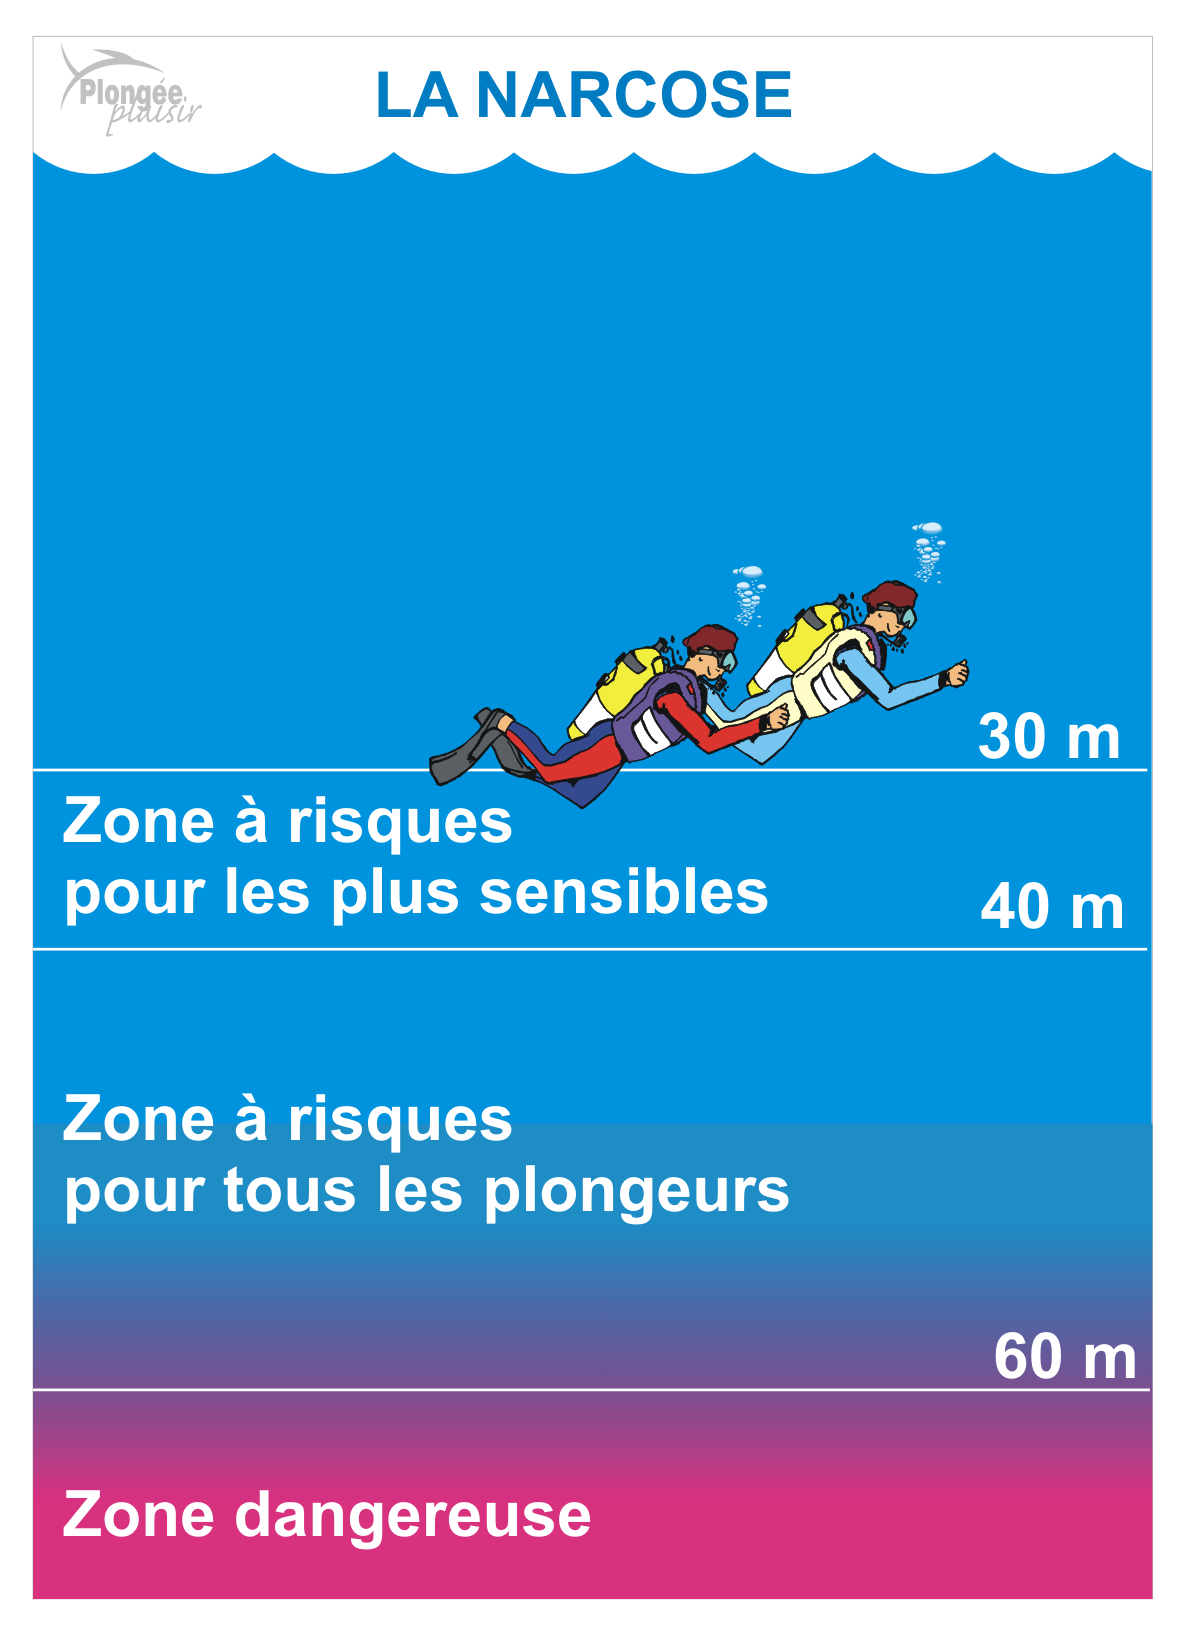
\includegraphics[height=0.85\textheight, keepaspectratio]{images/zones_narcose.png}
            \end{center}
        \end{column}
    \end{columns}
\end{frame}

\begin{frame}{Narcose — Symptômes et Signes}
    \textbf{Les Effets (souvent masqués) :}
    \begin{itemize}
        \item Troubles de la mémoire immédiate, retard de réaction, lecture répétée des instruments.
        \item Euphorie ou anxiété légère, vision tunnel.
        \item Le plongeur ne se rend souvent compte de rien.
    \end{itemize}

    \textbf{La Crise (\textcolor{ffessmred}{Danger}) :}
    \begin{itemize}
        \item Comportement aberrant (croire remonter alors qu'on descend).
        \item Incapacité à communiquer avec la palanquée.
        \item Absence de réponse aux signes.
    \end{itemize}
\end{frame}

\begin{frame}{Narcose — Prévention et CAT}
    \textbf{Prévention (Spécifique N3) :}
    \begin{itemize}
        \item \textbf{\textcolor{ffessmred}{Accès progressif}} à la profondeur (surtout en début de saison).
        \item Bonne forme physique, pas de stress, pas de médicaments.
        \item Descente \textbf{\textcolor{ffessmred}{maîtrisée}} (repères visuels).
    \end{itemize}

    \textbf{Conduite à Tenir (CAT) :}
    \begin{enumerate}
        \item \textbf{Si simples effets :} \textcolor{ffessmred}{Remonter de quelques mètres} (\textbf{10 à 15 mètres}) pour faire disparaître les troubles.
        \item \textbf{Si CRISE avérée :}
        \begin{itemize}
            \item \textbf{INTERVENTION IMMÉDIATE} du binôme.
            \item \textbf{\textcolor{ffessmred}{FIN DE PLONGÉE}} obligatoire.
            \item \textbf{Remontée assistée} vers la surface.
            \item Surveillance post-plongée (cas extrêmes).
        \end{itemize}
    \end{enumerate}
\end{frame}

\begin{frame}{L'Hypercapnie (Essoufflement) — Cause \& Mécanisme}
    \begin{columns}[T,totalwidth=\textwidth]
        \column{0.55\textwidth}
        \textbf{\textcolor{ffessmred}{Cause}} :
        \begin{itemize}
            \item Excès de \textbf{$CO_2$} (dioxyde de carbone).
            \item Souvent dû à un \textbf{effort excessif} inadapté à la profondeur ou une \textbf{mauvaise ventilation}.
        \end{itemize}

        \vspace{0.5em}
        \textbf{\textcolor{ffessmred}{Mécanisme}} :
        \begin{itemize}
            \item Augmentation du $CO_2$ dans le sang.
            \item Stimulation des centres respiratoires $\rightarrow$ besoin d'air.
            \item \textbf{Cercle vicieux} : Ventilation inefficace $\rightarrow$ $CO_2$ augmente $\rightarrow$ Fréquence s'accélère.
        \end{itemize}

        \column{0.45\textwidth}
        \centering
        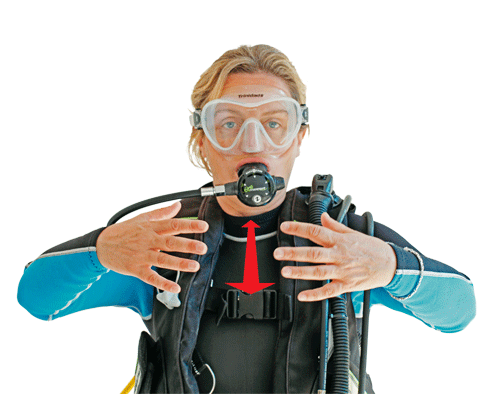
\includegraphics[height=0.7\textheight, keepaspectratio]{images/signes_essoufflement.png}
    \end{columns}
\end{frame}

\begin{frame}{L'Hypercapnie (Essoufflement) — Symptômes \& Facteurs}
    \textbf{\textcolor{ffessmred}{Symptômes}} :
    \begin{itemize}
        \item Ventilation \textbf{rapide} et \textbf{superficielle} (halètement).
        \item Sentiment d'\textbf{étouffement}, angoisse ("soif d'air").
        \item Risque de panique et d'accident grave (noyade, surpression).
    \end{itemize}

    \vspace{0.8em}
    \textbf{\textcolor{ffessmred}{Facteurs favorisants}} :
    \begin{itemize}
        \item \textbf{Matériel} : Détendeur dur/mal réglé, combinaison trop serrée.
        \item \textbf{Physique} : Froid, Stress, mauvaise condition physique.
        \item \textbf{Profondeur} : La densité de l'air augmente l'effort ventilatoire (\textit{attention à 60m !}).
        \item \textbf{Effort} : Palmage intensif contre courant.
    \end{itemize}
\end{frame}

\begin{frame}{Essoufflement — Prévention \& CAT}
    \begin{block}{Le risque associé}
        L'essoufflement augmente l'accumulation de CO$_2$ et le risque d'\textbf{ADD} 
        (accélération circulatoire $\rightarrow$ accélération ventilatoire = saturation accrue).
    \end{block}

    \vspace{0.5em}
    \begin{columns}[T,totalwidth=\textwidth]
        \column{0.48\textwidth}
        \textbf{\textcolor{ffessmred}{Prévention N3}}
        \begin{itemize}
            \item \textbf{Adapter l'effort} à la profondeur (la densité de l'air augmente).
            \item \textbf{Matériel} adapté et entretenu (détendeur, lestage).
            \item \textbf{Expiration} active et profonde.
            \item Se protéger du froid et du stress.
        \end{itemize}

        \column{0.48\textwidth}
        \textbf{\textcolor{ffessmred}{Conduite à Tenir (CAT)}}
        \begin{itemize}
            \item \textbf{\textcolor{ffessmred}{STOP}} : Arrêter tout effort immédiatement.
            \item \textbf{\textcolor{ffessmred}{Signaler}} : Prévenir le binôme.
            \item \textbf{\textcolor{ffessmred}{Ventiler}} : Se forcer à expirer à fond.
            \item Si persistant : \textbf{Assistance} et \textbf{remontée} (fin de plongée).
        \end{itemize}
    \end{columns}
\end{frame}

\begin{frame}{Essoufflement — Autonomie et adaptation au Binôme et au Milieu}
    \small
    En autonomie, l'adaptation est la clé de la sécurité.
    \vspace{0.4em}
    
    \begin{columns}[T,totalwidth=\textwidth]
        \column{0.48\textwidth}
        \textbf{Le Facteur Humain (Binôme)}
        \begin{itemize}
            \item Chaque plongeur réagit différemment (technique, condition physique).
            \item Un équipier peut se fatiguer plus vite que l'autre (souvent dû à une \textbf{\textcolor{ffessmred}{vitesse de déplacement}} excessive).
            \item \textbf{Règle} : Le rythme de la palanquée est celui du plus lent / moins expérimenté.
        \end{itemize}

        \column{0.48\textwidth}
        \textbf{Adaptation au Milieu (Courant)}
        \begin{itemize}
            \item \textbf{Surface} : Utiliser une \textbf{ligne de vie} si courant.
            \item \textbf{Immersion} : Se tenir au \textbf{mouillage} pour éviter la dérive.
            \item \textbf{Fonds} : Modifier le parcours pour s'\textbf{abriter derrière le relief}, éviter la lutte contre le courant.
        \end{itemize}
    \end{columns}

    \begin{block}{Anticipation}
        Ces stratégies doivent être définies lors du \textbf{briefing}, avant la mise à l'eau.
    \end{block}
\end{frame}
\section{L'Œdème Pulmonaire d'Immersion (OPI)}

\begin{frame}{Mécanisme de l'OPI}
  \begin{columns}[c]
    \begin{column}{0.55\textwidth}
      \begin{block}{Définition}
        Inondation brutale des alvéoles par du \textbf{plasma sanguin}.
        \small{Ce n'est pas une entrée d'eau, mais une fuite interne.}
      \end{block}
      
      \textbf{Le mécanisme physiologique :}
      \begin{enumerate}
        \item Immersion $\Rightarrow$ \textbf{Blood Shift} (sang chassé vers le thorax).
        \item Augmentation de la pression dans les capillaires pulmonaires.
        \item Rupture de la \textbf{barrière alvéolo-capillaire}.
      \end{enumerate}
    \end{column}
    
    \begin{column}{0.45\textwidth}
      \centering
      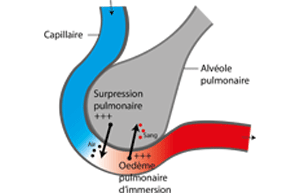
\includegraphics[width=\textwidth]{images/infos-opi}
      \tiny{\textit{Passage du plasma vers l'alvéole (Défaillance barrière)}}
    \end{column}
  \end{columns}
\end{frame}

\begin{frame}{Facteurs favorisants (Le profil à risque)}
  Contrairement à la surpression, l'OPI est souvent lié à la condition du plongeur.
  
  \begin{alertblock}{Facteurs aggravants (Cumulatifs)}
    \begin{itemize}
      \item \textbf{Froid} (Vasoconstriction périphériques).
      \item \textbf{Effort physique} important (palmage soutenu).
      \item \textbf{Hypertension artérielle} (HTA) et problèmes cardiaques.
      \item \textbf{Stress} (Augmentation rythme cardiaque).
    \end{itemize}
  \end{alertblock}

  \begin{block}{Autre facteur identifié}
    \begin{itemize}
      \item Âge (> 40-50 ans).
    \end{itemize}
  \end{block}
\end{frame}

\begin{frame}{Symptômes et Conduite à tenir}
  \begin{columns}[T]
    \begin{column}{0.45\textwidth}
      \textbf{Symptômes :}
      \begin{itemize}
        \item Sensation d'étouffement, dyspnée.
        \item \textbf{Toux} irrésistible pendant la plongée.
        \item Bruits respiratoires (gargouillis).
        \item \textbf{Crachats mousseux et rosés} (Hémoptysie).
      \end{itemize}
      
      \begin{alertblock}{Aggravation}
        Les symptômes \textbf{s'aggravent à la remontée}.
      \end{alertblock}
    \end{column}
    
    \begin{column}{0.45\textwidth}
      \begin{block}{Conduite à tenir}
        \begin{enumerate}
          \item \textbf{Arrêt de tout effort} immédiat.
          \item Remontée assistée calme (éviter la panique).
          \item En surface : Oxygénothérapie (O$_2$).
          \item Appel des secours (CROSS/VHF) $\Rightarrow$ \alert{\textbf{URGENCE VITALE}}.
        \end{enumerate}
      \end{block}
    \end{column}
  \end{columns}
\end{frame}
\input{slides/9-le-froid}
\section{Organisation et Planification}

\begin{frame}{Organiser une plongée en autonomie}
    Le N3 peut plonger sans Directeur de Plongée (DP). Il est responsable de l'organisation.
    
    \textbf{Les étapes clés :}
    \begin{enumerate}
        \item Vérifier la \textbf{Météo} (Vents, Houle, Météo France, Apps, CROSS).
        \item Choisir le \textbf{Site} (Profil, niveau des plongeurs, zones interdites).
        \item Préparer le \textbf{Bateau} (Carburant, Mouillage, VHF testée).
        \item Établir la \textbf{Fiche de Sécurité} (Palanquées, paramètres prévus).
    \end{enumerate}
\end{frame}

\begin{frame}{La Météo — Sources d'Information}
    Il existe plusieurs moyens de vérifier la météo avant le départ :
    
    \begin{itemize}
        \item \textbf{Internet} : Sites web spécialisés (Météo France, Lamma, etc.).
        \item \textbf{Applications} : Sur smartphone (Windy, Maree.info, etc.).
        \item \textbf{Capitainerie} : Affichages au port ou renseignement direct.
        \item \textbf{Message Radio du CROSS} (VHF) :
        \begin{itemize}
            \item Se renseigner sur les \textbf{horaires} de diffusion.
            \item Connaître les \textbf{canaux} de diffusion (VHF).
        \end{itemize}
    \end{itemize}
    \centering
    
\includegraphics[height=0.25\textheight, keepaspectratio]{images/meteo} 
\end{frame}

\begin{frame}{Le Choix du Site de Plongée}
    \textbf{Le site se choisit en fonction :}
    \begin{itemize}
        \item Des \textbf{conditions météo}.
        \item Du \textbf{profil} (profondeur, courant potentiel...).
        \item Des \textbf{envies} et de l'\textbf{état physique} des plongeurs.
    \end{itemize}
    
    \vspace{0.8em}
    \textbf{Points de vigilance :}
    \begin{itemize}
        \item Faire attention aux \textbf{zones interdites} (réserves, zones militaires...) indiquées sur les \textbf{cartes marines}.
        \item \textbf{Informer une personne à terre} du lieu choisi et des horaires prévus avant le départ (pour déclencher les secours en cas de retard anormal).
    \end{itemize}
\end{frame}

\begin{frame}{Matériel de Sécurité Obligatoire (Bateau)}
    En tant que responsable, vérifier la présence du matériel (Art. A.322-78-2):
    \begin{columns}[totalwidth=\textwidth]
        \column{0.5\textwidth}
        \textbf{Secours \& Médical :}
        \begin{itemize}
            \item Trousse de secours complète.
            \item Oxygénothérapie (Bavu + O2).
            \item Eau douce potable.
            \item Couverture isothermique.
            \item Fiches d'évacuation.
        \end{itemize}

        \textbf{Opérationnel \& Signalisation :}
        \begin{itemize}
            \item Moyen de communication (VHF).
            \item Bouteille de secours (détendeur monté).
            \item Tables de plongée (immergables).
            \item \textbf{Pavillon Alpha}.
        \end{itemize}
        \vspace{0.5em}
        \column{0.5\textwidth}
        \centering
        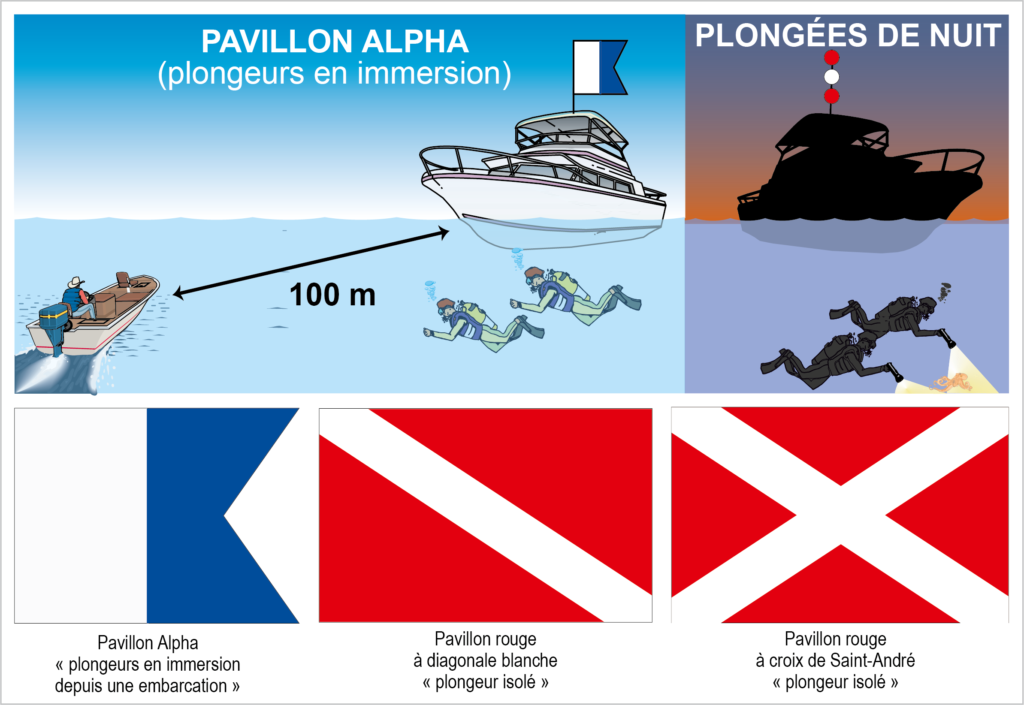
\includegraphics[width=0.9\columnwidth, keepaspectratio]{images/signalisation-plongeurs.png}
    \end{columns}
\end{frame}

\begin{frame}{Procédures d'Urgence — Alerte}
    \textbf{Alerte (CROSS - VHF Canal 16 ou Tél 196)} :
    \begin{itemize}
        \item Message \textbf{PAN-PAN} (Urgence relative) ou \textbf{MAYDAY} (Détresse vitale).
        \item Donner dans l'ordre :
        \begin{enumerate}
            \item \textbf{Position} du navire.
            \item \textbf{Nature} du problème (ADD, Noyade...).
            \item \textbf{Nombre} et état des victimes.
        \end{enumerate}
    \end{itemize}
\end{frame}

\begin{frame}{Plan de Secours}
    \centering
    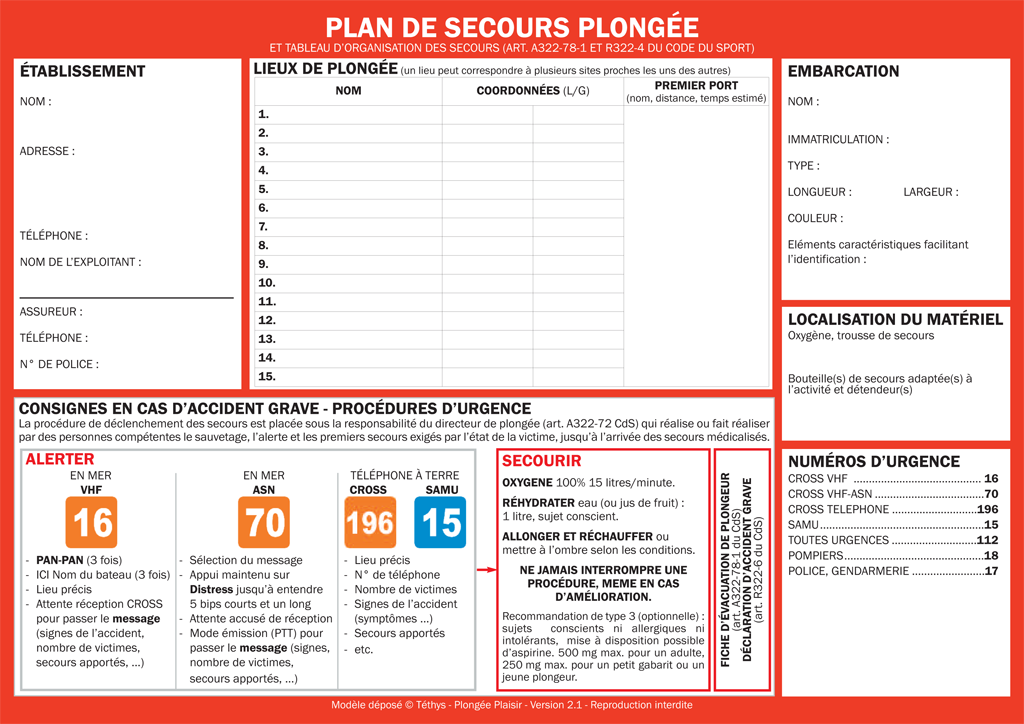
\includegraphics[width=\textwidth, height=0.87\textheight, keepaspectratio]{images/plongee_plaisir_plan_secours.png}
\end{frame}

\begin{frame}{Fiche d'Évacuation}
    \centering
    % Plan d'organisation ou cartographie large
    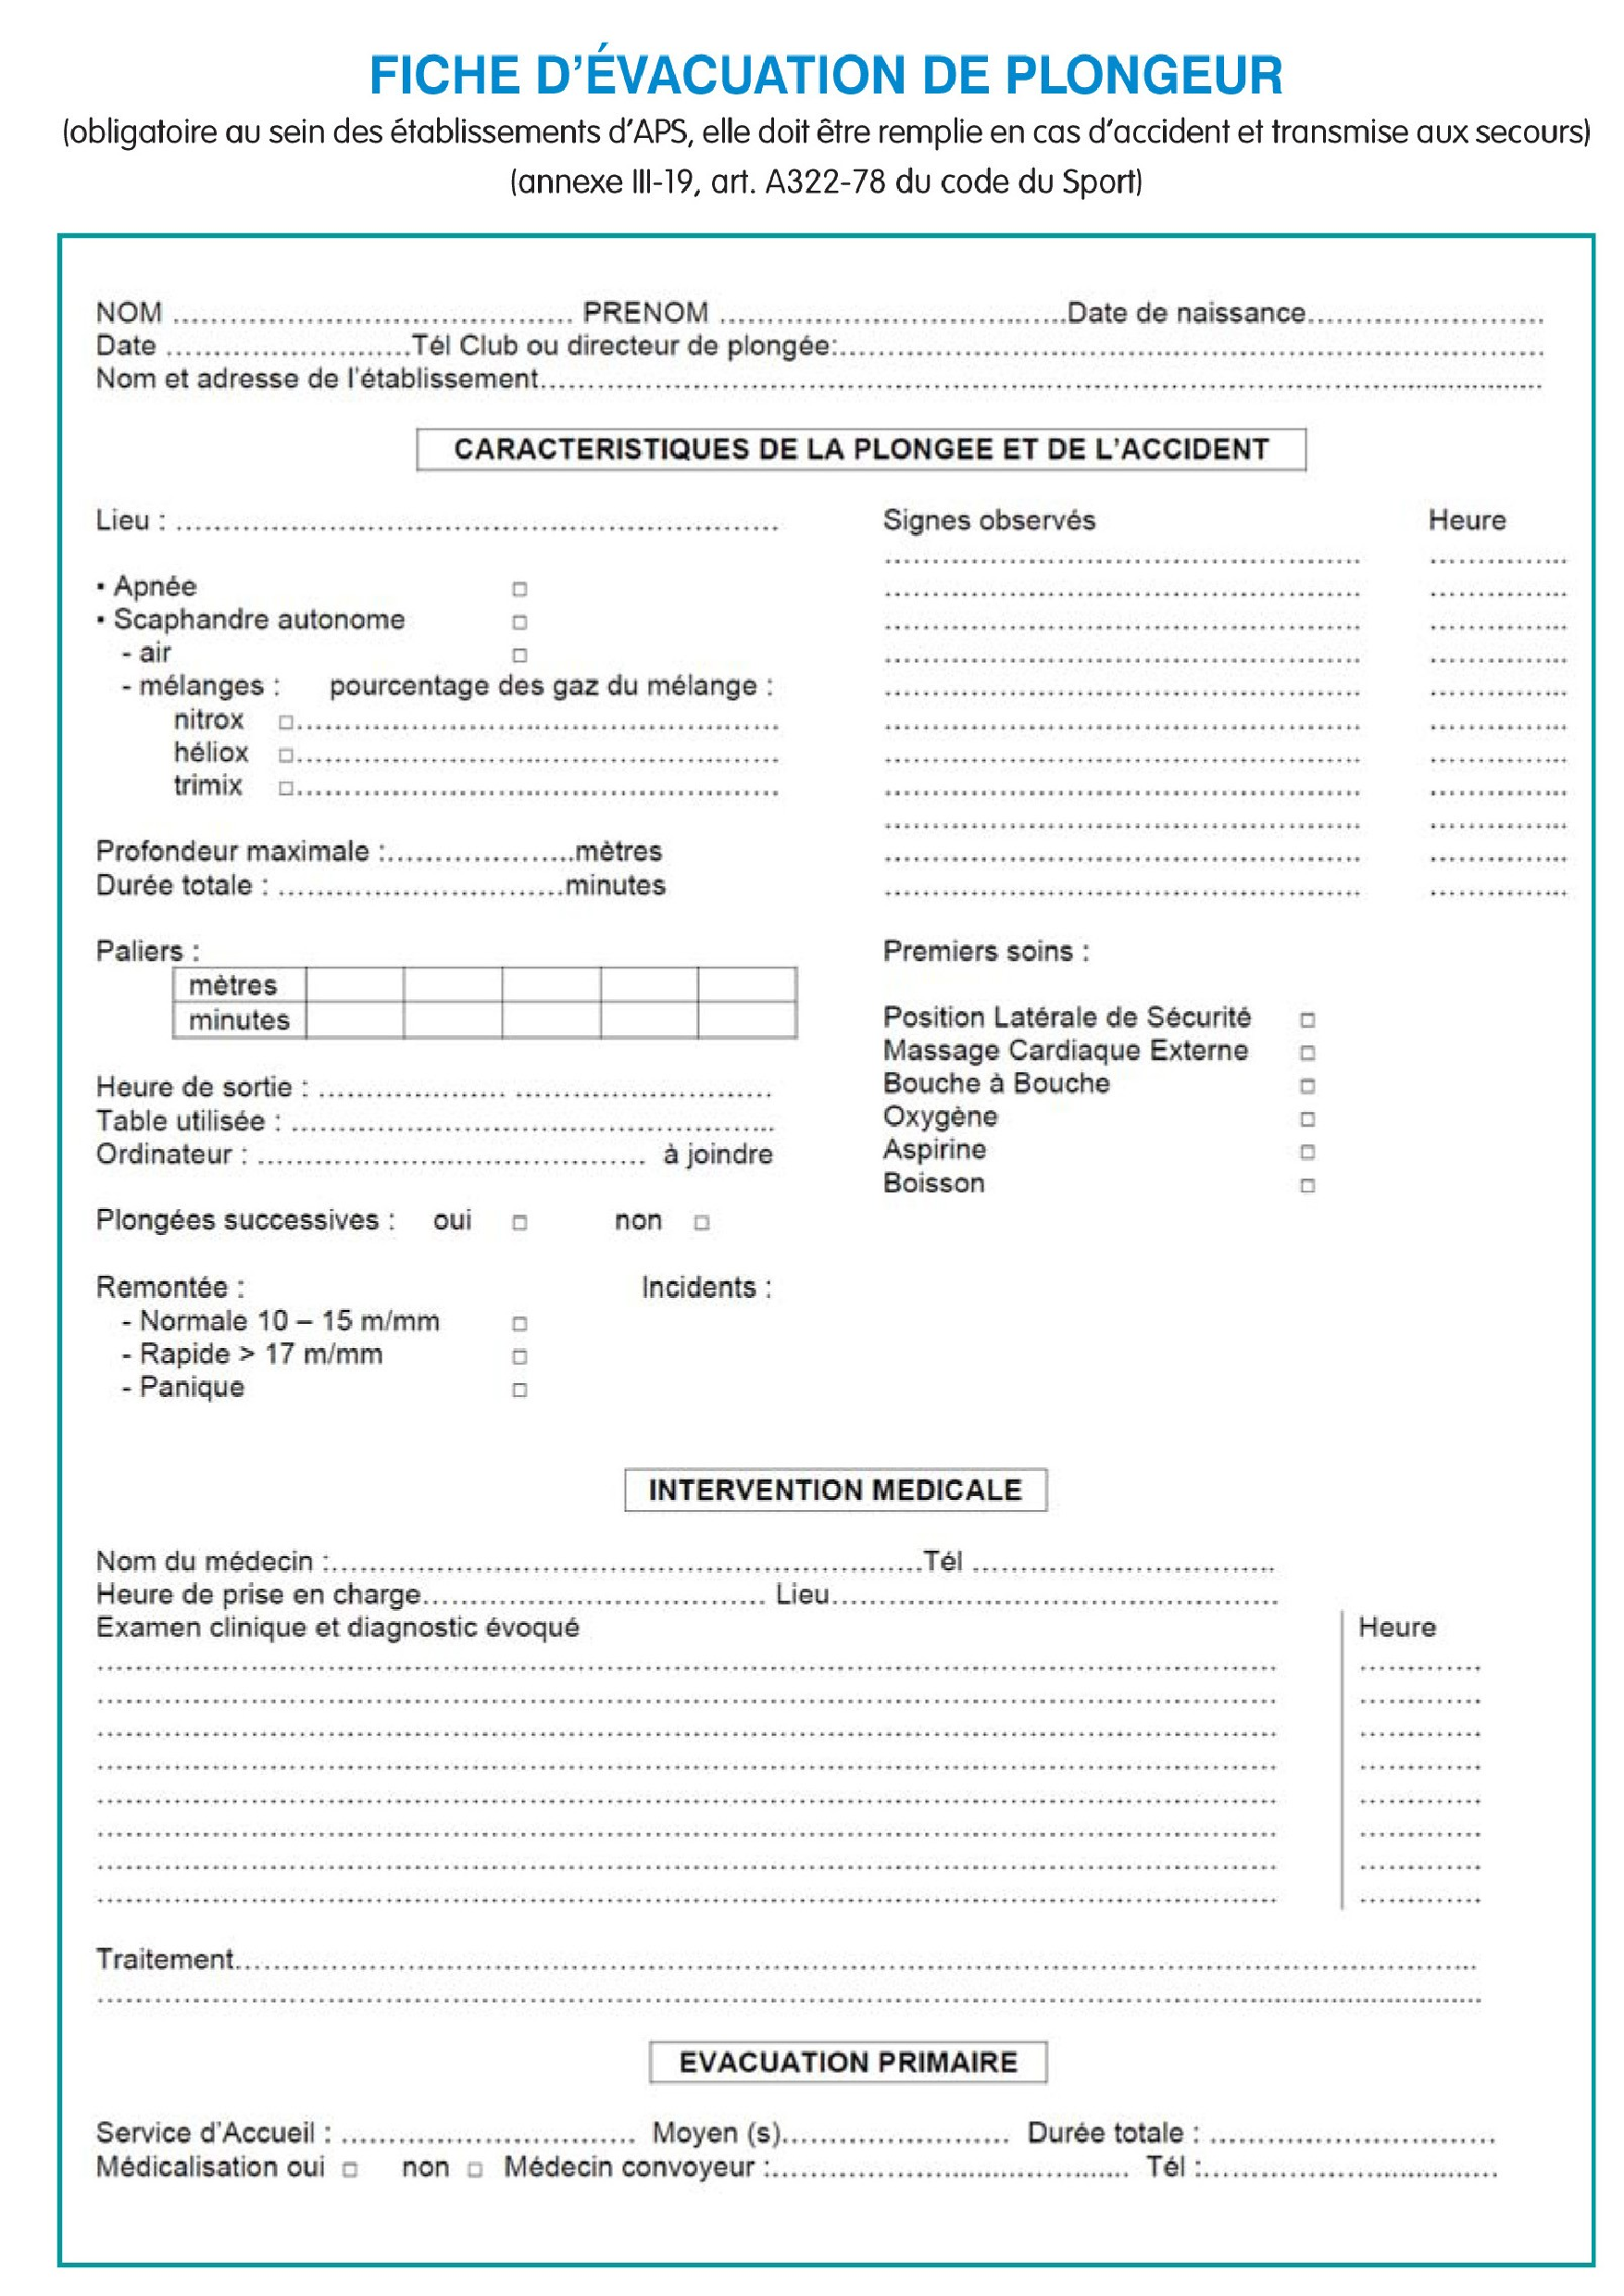
\includegraphics[height=0.85\textheight, keepaspectratio]{resources/pdf/fiche_d_evacuation.pdf}
\end{frame}

\begin{frame}{Organiser les Mises à l'Eau}
    \textbf{Logistique}
    \begin{itemize}
        \item Adapter le mouillage au profil (éviter si roches profondes ou houle).
    \end{itemize}

    \begin{alertblock}{Sécurité de Surface (Impératif)}
        \begin{itemize}
            \item \textbf{Pilote à bord} : Une personne compétente reste en surface.
            \item \textbf{Alternative} : Plongée \textbf{« en décalé »} (une palanquée assure la sécu pendant que l'autre plonge).
        \end{itemize}
    \end{alertblock}

    \vspace{0.5em}
    \textbf{Avant l'immersion}
    \begin{itemize}
        \item Remplir la \textbf{Fiche de Sécurité} (Noms, Aptitudes, Paramètres).
        \item \textbf{Vérification mutuelle} : Connaître l'équipement du binôme.
    \end{itemize}
\end{frame}

\begin{frame}{Fiche de Sécurité}
    \centering
    % Fiche de sécurité obligatoire pour le DP/Responsable
    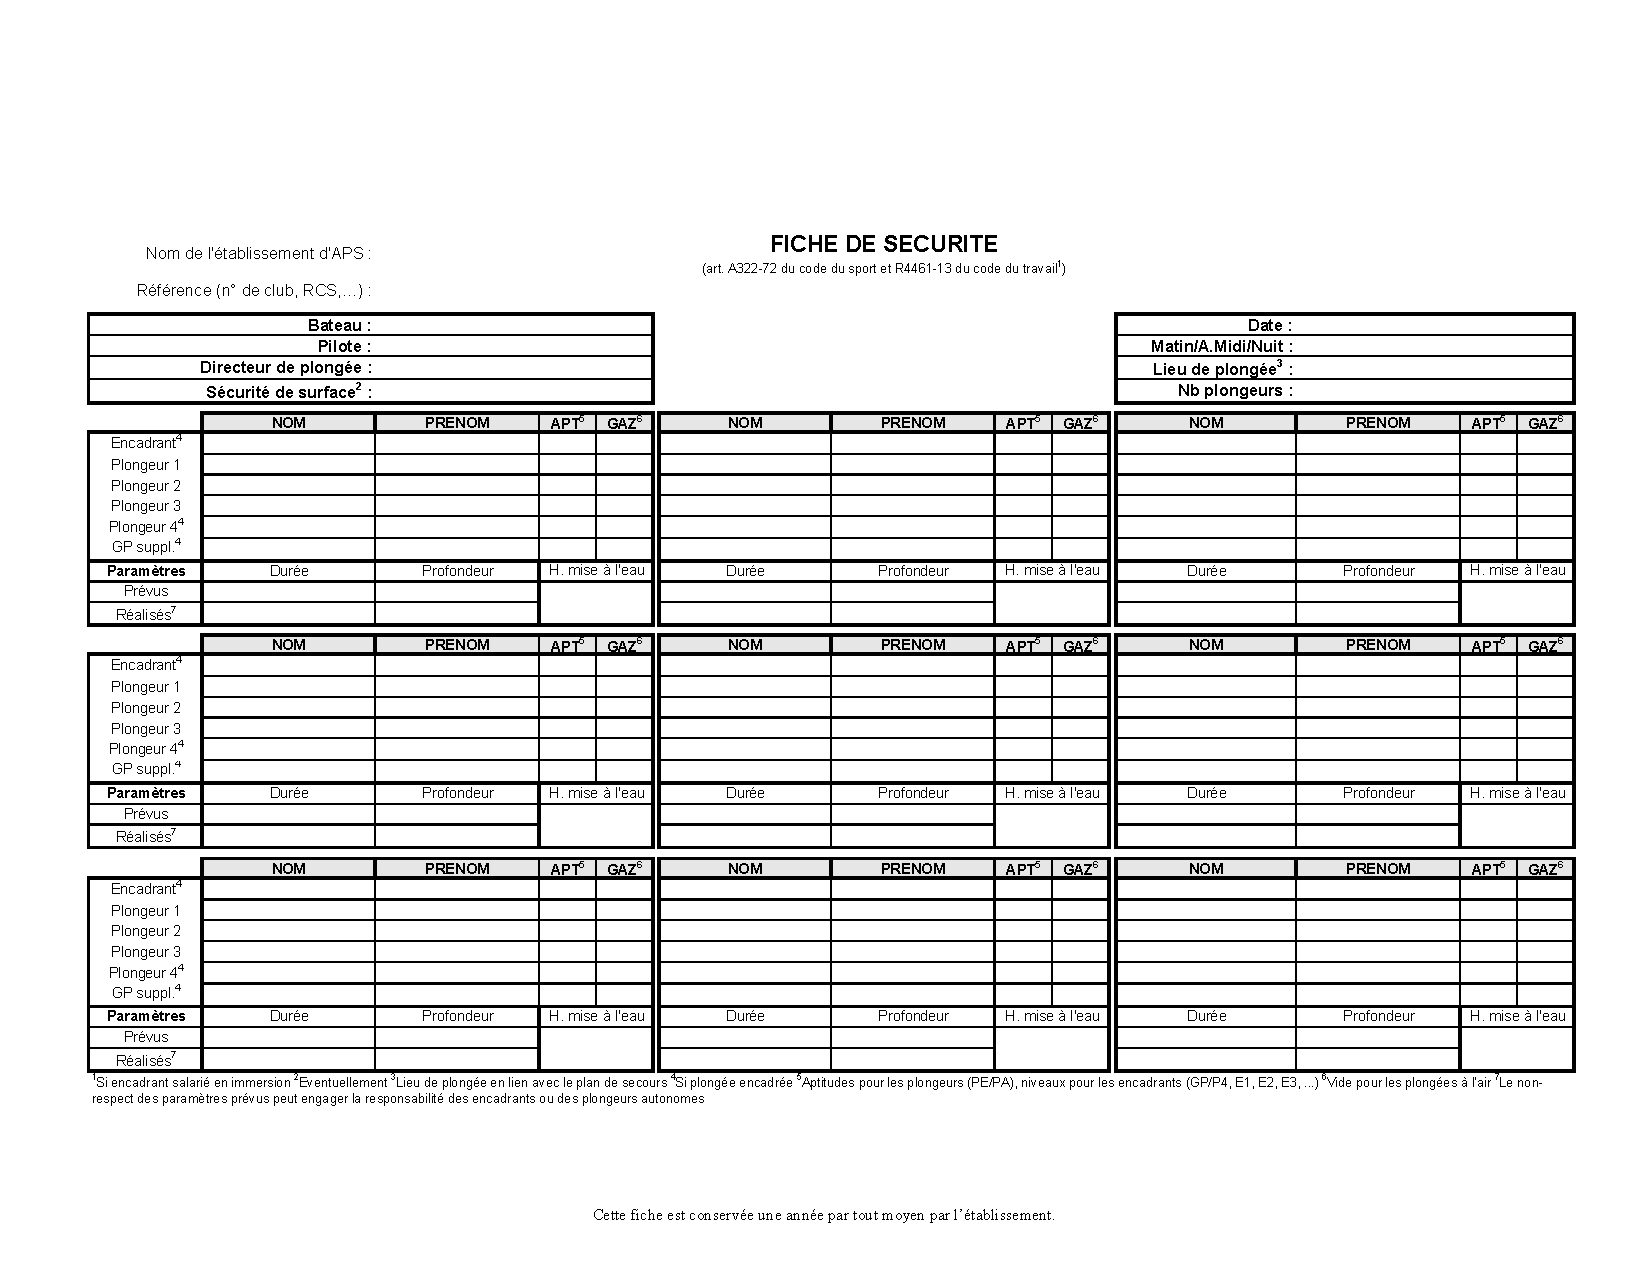
\includegraphics[height=\textheight, keepaspectratio,trim={0 0 0 3.9cm}, clip]{resources/pdf/fiche_de_securite.pdf}
\end{frame}

\begin{frame}{Matelotage — Nœuds utiles}
    \textbf{Savoir nouer est essentiel en bateau :}
    
    \vspace{0.5em}
    \begin{columns}[T,totalwidth=\textwidth]
        \column{0.5\textwidth}
        \textbf{Nœud de Chaise}
        \begin{itemize}
            \item Boucle fixe qui ne glisse pas.
            \item Idéal pour s'amarrer sur un anneau ou hisser du matériel.
        \end{itemize}
        \centering
        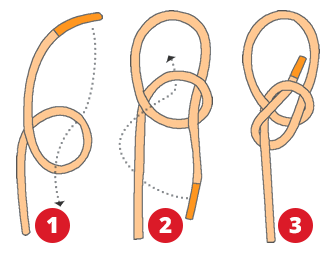
\includegraphics[height=0.4\textheight, keepaspectratio]{images/noeud-chaise.png}

        \column{0.5\textwidth}
        \textbf{Nœud de Cabestan}
        \begin{itemize}
            \item Nœud d'accroche rapide.
            \item Pour amarrer temporairement (autobloquant sous tension).
        \end{itemize}
        \centering
        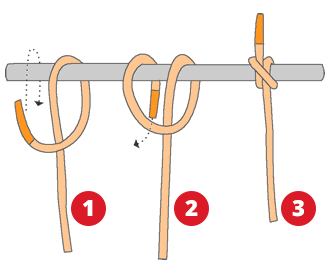
\includegraphics[height=0.4\textheight, keepaspectratio]{images/cabestan.png}
    \end{columns}
\end{frame}

\begin{frame}{Planification de la Palanquée}
    Avant la mise à l'eau, la palanquée doit se mettre d'accord sur:
    \begin{itemize}
        \item La \textbf{Profondeur Maximum}.
        \item La \textbf{Durée Maximum} (ou DTR max).
        \item La pression de décollage (réserve d'air).
        \item Le protocole de décompression (quel ordinateur suit-on ?).
        \item Les signes de communication spécifiques.
    \end{itemize}
    
    \begin{center}
        \textit{Plonger en autonomie, c'est plonger responsable !}
    \end{center}
\end{frame}
\input{slides/11-outils-decompression}
\input{slides/12-conclusion}

\end{document}
